\documentclass[10pt,twocolumn,letterpaper]{article}
%\usepackage[latin1]{inputenc}

%\usepackage{url}
%\usepackage{booktabs}

\usepackage{cvpr}
\usepackage{times}
\usepackage{epsfig}
\usepackage{graphicx}
\usepackage{amsmath}
\usepackage{amssymb}
\usepackage{amsmath}
\usepackage{amsfonts}
\usepackage{subfigure}
\usepackage{nonfloat}
\usepackage{url}
\usepackage[colorlinks=true, linkcolor=green, pagebackref]{hyperref}
\usepackage{textcomp} % for textonehalf
%\usepackage{subfig}
%\usepackage{subref}
\graphicspath{{imgs/}}

\usepackage{xspace}
\renewcommand*{\eg}{e.g.\@\xspace}
\renewcommand*{\ie}{i.e.\@\xspace}
\newcommand*{\ea}{et al.\@\xspace}
\renewcommand*{\vs}{vs.\@\xspace}
%\renewcommand{\arraystretch}{1.5}

%\cvprfinalcopy % *** Uncomment this line for the final submission

\def\cvprPaperID{****} % *** Enter the CVPR Paper ID here
\def\httilde{\mbox{\tt\raisebox{-.5ex}{\symbol{126}}}}

% General notation
\newcommand{\prob}{Pr}
\newcommand{\degree}{^{\circ}}

% Image notation
\newcommand{\rgbdimage}{\mathcal{D}}
\newcommand{\intrinsics}{K}
\newcommand{\pixelidx}{\gamma}
\newcommand{\edgeimidx}{\xi}

% Voxel notation
\newcommand{\voxelgrid}{\mathcal{V}}
\newcommand{\voxel}{v}
\newcommand{\voxidx}{i}
\newcommand{\voxelidxs}{m, n, l}

% Point cloud notation
\newcommand{\project}{\mathbf{p}}
\newcommand{\pcloud}{\mathcal{P}}
\newcommand{\point}{\mathbf{p}}
\newcommand{\normal}{\mathbf{n}}
\newcommand{\updir}{\mathbf{u}}

% Transformations
\newcommand{\trans}{T}
\newcommand{\extrinsics}{H}
\newcommand{\voxelgridtoworld}{\trans_{\voxelgrid \rightarrow w}}


\definecolor{red}{rgb}{0.95,0.4,0.4}
\definecolor{blue}{rgb}{0.4,0.4,0.95}
\definecolor{darkred}{rgb}{0.8,0,0}
\definecolor{darkgreen}{rgb}{0,0.5,0}
\definecolor{grey}{rgb}{0.6,0.6,0.6}

\newcommand{\todo}[1]{\textcolor{red}{TODO: #1}}
\newcommand{\note}[1]{\textcolor{blue}{NOTE: #1}}
\newcommand{\status}[1]{\textcolor{blue}{Status: #1}}
\newcommand{\add}[1]{\textcolor{darkgreen}{#1}}
\newcommand{\remove}[1]{\textcolor{grey}{#1}}



%[citecounter=true, style=ieee]
%\usepackage{biblatex}
%\addbibresource{bibtex/strings.bib}
%\addbibresource{bibtex/main.bib}
%\addbibresource{bibtex/crossrefs.bib}
%addbibresource{\jobname.bib}


\title{Structured Prediction of Unobserved Voxels From a Single Depth Image}

%\author{Michael Firman, Gabriel Brostow, Simon Julier \ea}

\begin{document}


\maketitle

\begin{abstract}
	%Building a representation of the geometry of a scene is an essential task for many applications including robotic navigation, scene re-lighting and object manipulation. 
	%Most existing works to recover the scene geometry rely on combining multiple views of the scene captured from many different directions or use of \emph{a priori} information about the expected semantic make-up of the scene.

  Building a complete 3D model of a scene is underconstrained from a single camera view.
  To gain a full volumetric model from a single view we typically either need lots of data or to work under the strong assumption that we have a library of training instances that we can use to model the shape of each object in the scene.
  
  We hypothesise that objects of dissimilar semantic classes often share similar shapes, enabling a limited  training dataset to model the shape of a wide range of objects and hence estimate the hidden geometry of various scenes.
  Under this hypothesis we have implemented a system which can complete the unobserved geometry of a scene using a library of volumetric elements learned from training data.
  Using a novel feature representation, we train our model to map from observed depth values to voxel occupancy in the region surrounding a 3D location.
  Through a prototype system we valid our approach qualitatively and quantitatively on a range of indoor scenes.


%	Our primary contribution is the \emph{voxlet}, a primitive explaining voxel occupancy in the region of a point in 3D space. We also develop a novel feature representation, which coupled with a Random Forest forms a mapping from a point in a depth image to a prediction of voxel occupancy in the point's vicinity.
 % We present a range of qualitative and quantitative results which show we can accurately reconstruct shape in both simple and challenging scenes, and we show many advantages over the current state-of-the-art.
%  We demonstrate the advantages of our technique over the current state of the art.

  %, method comprises of three main components:
   % 1) We generate a dinctionary of voxlets, which is a primitive describing 
   % 2) We introduce a novel regional feature to describe the shape of the region surrounding a point.
    %3) We use a Random Forest, trained on turntable and real-world data to map our feature representations of a pixel to a suitable voxlet which can be used to describe local voxel occupancy.
    %4) Finally we combine and regularise the  predictions to form a full probabilistic distribution of occupancy for each voxel in the scene, respecting constraints such as connectivity and gravity.

\end{abstract}

%%%%%%%%%%%%%%%%%%%%%%%%%%%%%%%%%%%%%%%%%%%%%%%%%%%%%%%%%%%%%%
\section{Introduction}
\footnote{Potential to add to intro: Psychology: Are humans good at this? Not much evaluation in other work.}
%%%%%%%%%%%%%%%%%%%%%%%%%%%%%%%%%%%%%%%%%%%%%%%%%%%%%%%%%%%%%%


% What is the problem?
We broadly categorize space in our world as being `occupied' and opaque, or `vacant' and transparent.
Depth cameras such as the Microsoft Kinect are able to give an estimate of which regions of a scene are composed of free, vacant space.
However, each pixel in a depth image only makes a estimate of occupancy until the first solid surface is encountered along that camera ray (figure \ref{fig:intro}).
The `occlusion phenomenon' prevents any information from being extracted about the occupancy of space beyond that first surface.

% Why is it interesting and important?
There are many applications, however, which crucially require a complete representation of the world geometry.
When a robot sets out to grasp an unknown object in an unknown scene a 3D model is required to prevent collision with the object or nearby clutter.
Separately, in photo-editing, the full geometry could enable realistic shadows from a new light source to be automatically added to an image after it has been captured.

% Why is it hard? (E.g., why do naive approaches fail?)
Much research in computer vision has reconstructed the full 3D world from images of a scene captured from multiple viewpoints, thus overcoming the effect of occlusion  (\eg \cite{izadi-uist-2011}).
Instead, we focus on the task of classifying each voxel in a 3D scene as being either `occupied' or `vacant' given just a single depth image from one viewpoint.

% Why hasn't it been solved before? (Or, what's wrong with previous proposed solutions? How does mine differ?)
% What are the key components of my approach and results? Also include any specific limitations.

\newcommand{\introsubwidth}{0.48\columnwidth}
\begin{figure}[!t]
    \centering 
    \subfigure[Voxel world model]{%
        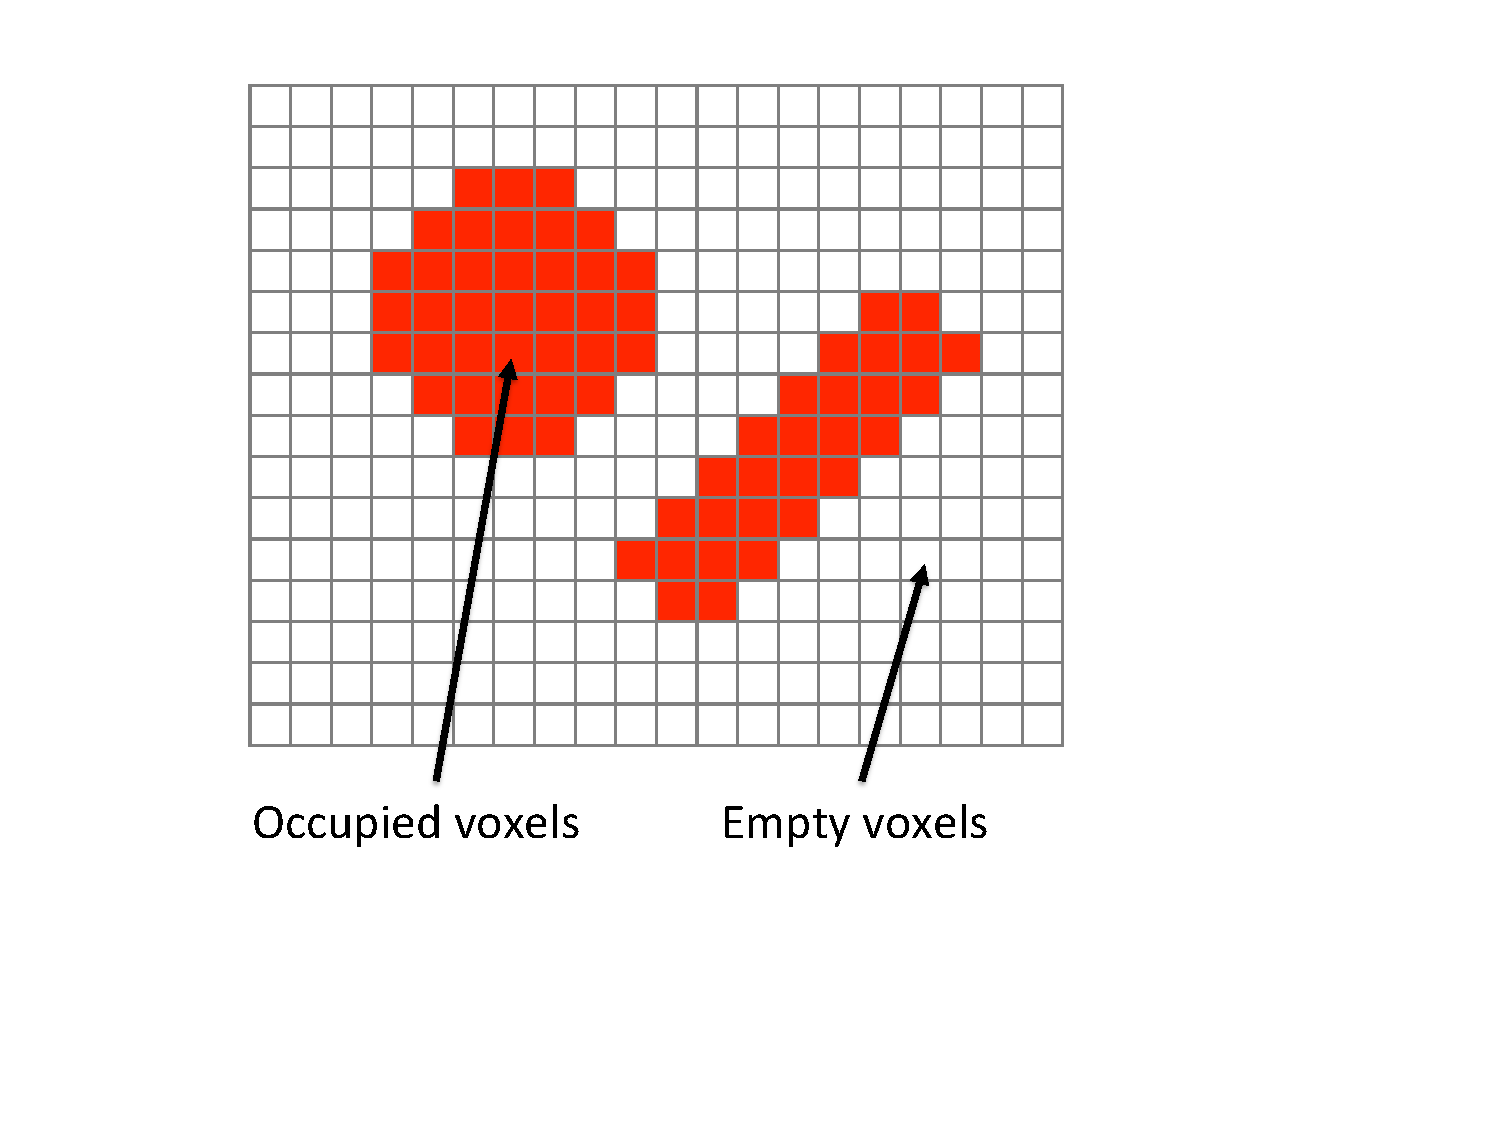
\includegraphics[width=\introsubwidth, clip=true, trim=110 105 205 30]{fig_1}}
        \hfill
    \subfigure[Depth rendering of world]{%
        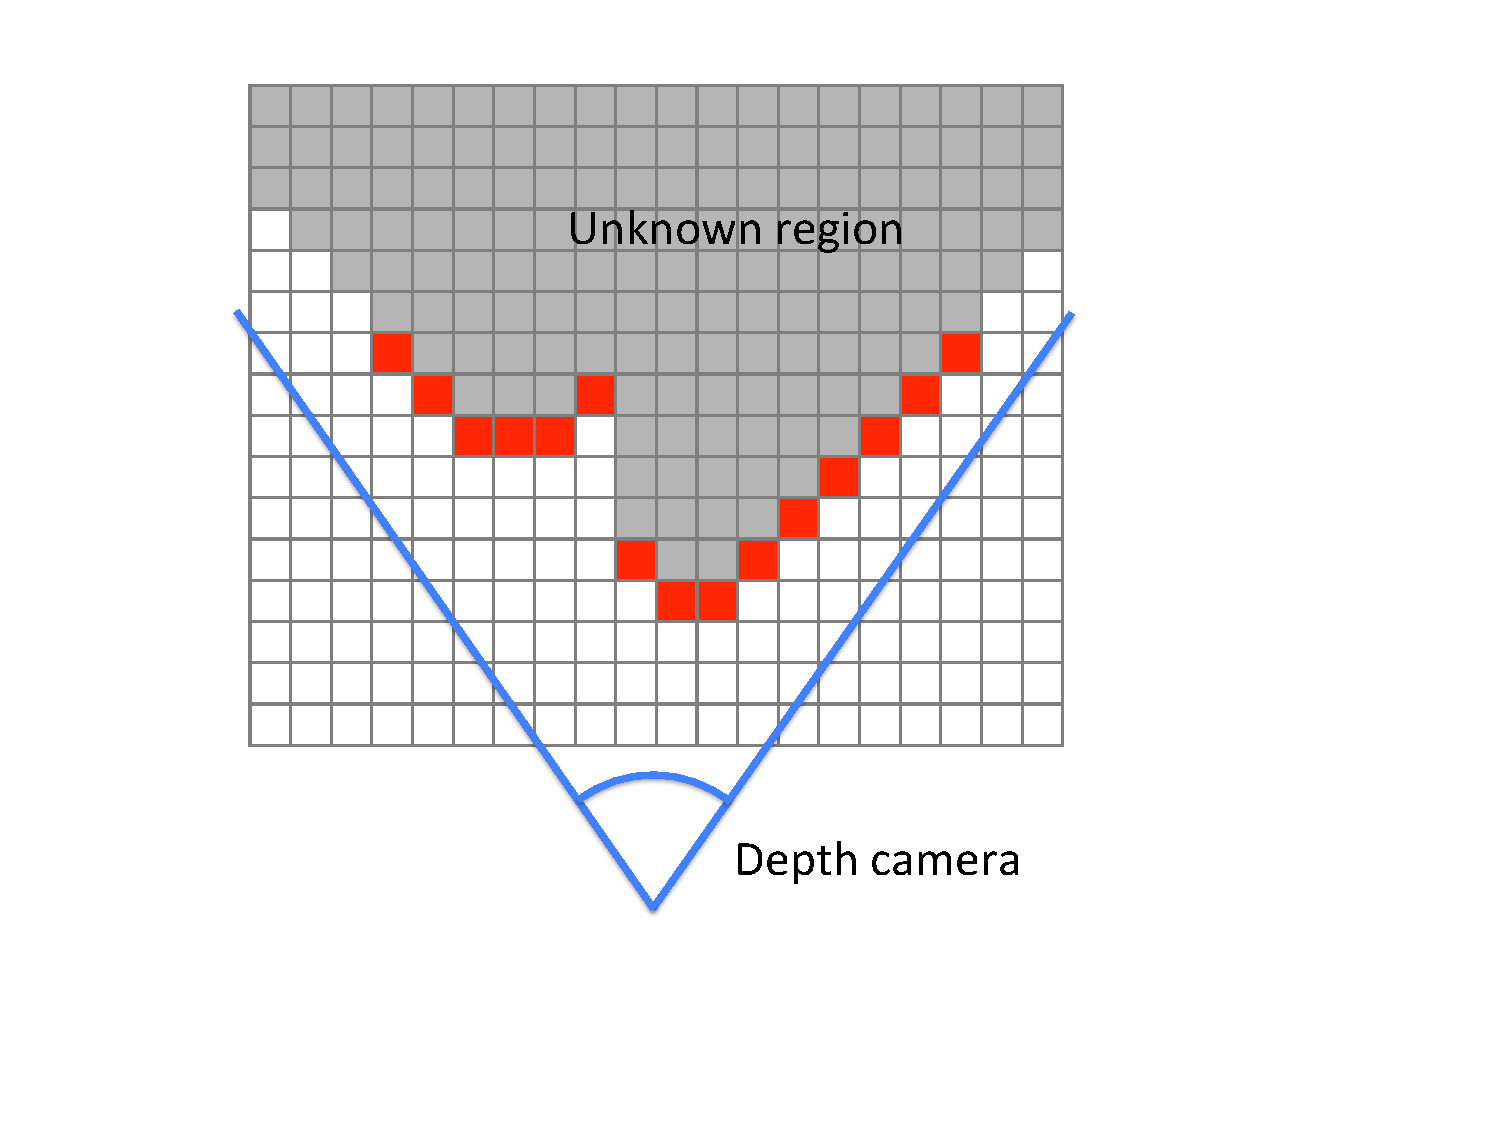
\includegraphics[width=\introsubwidth, clip=true, trim=110 105 205 30]{fig_1b}}
    \caption{
    We assume that our world is made up of voxels, which are either occupied or empty (vacant). 
    An overhead view of a coarse representation of this is shown in (a). 
    When observed by a depth camera, only the first visible voxel along each ray is seen.
    This leaves a region of unknown occupancy extending beyond the depth surface (b).
    The aim of our algorithm is to predict the state of the voxels in this unknown region.}%
    \label{fig:intro}
\end{figure}

%%%%%%%%%%%%%%%%%%%%%%%%%%%%%%%%%%%%%%%%%%%%%%%%%%%%%%%%%%%%%%
\subsection{Our approach and contributions}
%%%%%%%%%%%%%%%%%%%%%%%%%%%%%%%%%%%%%%%%%%%%%%%%%%%%%%%%%%%%%%

Given a single depth image, our system predicts whether each voxel in the scene is occupied by a solid impermeable object, or free and empty.
In effect, we strive to predict the voxelized occupancy grid of KinectFusion\footnote{\note{Actualy a TSDF...}} \cite{izadi-uist-2011}, but having test-time input of only a single view of the scene instead of multiple views.

We achieve this by learning a mapping from local and novel semi-regional features to a structured voxel occupancy prediction in the region of a query point, using a general-purpose collection of training objects and scenes.
We take inspiration from recent work which has segmented objects from images using silhouettes learned from different object classes \cite{kim-eccv-2012}.
Their work showed that shape can transcend class boundaries, enabling shape predictions to be made regardless of the accuracy of semantic classifiers.
Because we care about shape and voxel occupancy rather than semantic understanding, we are free to use training objects which differ from the objects being modeled in the scene.

Our key contributions are:

\begin{itemize}
\item \todo{Will fill these bullet points in final week}
\item \emph{Voxlets}, a representation of multi-voxel occupancy in the region of a point in a scene. 
We learn a dictionary of voxlets from training data, and at test time each predicted voxlet is able to make structured predictions about occupancy in the region of a query point.
\item We introduce a novel feature representation for a point in a depth image, which captures both local and region-level shape while respecting occlusions.
%\item Use of training data to allow our method to accurately complete detailed shapes.
\end{itemize}


%%%%%%%%%%%%%%%%%%%%%%%%%%%%%%%%%%%%%%%%%%%%%%%%%%%%%%%%%%%%%%
\section{Related work}
%%%%%%%%%%%%%%%%%%%%%%%%%%%%%%%%%%%%%%%%%%%%%%%%%%%%%%%%%%%%%%



%Most prior work in the area of completing missing data can be categorized according to its application domain (\eg meshes \cite{schnabel-eurographics-2009, ju-cst-2009}, 2D images \cite{gupta-cvpr-2011} or depth images \cite{shen-tog-2012}).


%\subsection{Taxonomy of related works}
Previous works on completing unknown regions of visual data can be categorized against several different criteria.
Some of these are given here, and we italicize the categories into which our approach falls.

Works can be classes according to their application domain, such as operating on meshes \cite{schnabel-eurographics-2009, ju-cst-2009}, 2D images \cite{gupta-cvpr-2011} or in \emph{voxel space} \cite{kim-iccv-2013}.
Some works make use of highly specialist hardware to capture images \eg \cite{velten-nature-2012}, while we use \emph{hardware available to consumers}.
Some approaches only aim to get a result that looks plausible, while we strive for \emph{accuracy in comparison to the ground truth}.
In comparison to works which use heuristics, we take a \emph{data-driven} approach to completion.
Data-driven approaches can be further classed according to whether the data used for completion comes from within the same image (\eg symmetry\cite{kroemer-humanoids-2012}) or from a \emph{database of training data}.

We now outline some of these previous approaches in more detail, and compare them to our approach.

%While some previous work on voxel occupancy prediction incorporates semantics, \eg \cite{kim-iccv-2013, shen-tog-2012, cocias-cgvcv-2013}, we are able to predict shape irrespective of recognition of semantic class.
\subsection{Fitting 3D models}
If prior knowledge is available about the objects present in the scene in the form of 3D models then an instance-level model can be fitted to a 3D scene.
This gives a good recovery of missing geometry of that object \cite{hinterstoisser-accv-2012, drost-3dimpvt-2012, rusu-iros-2010}.
Many advanced works focus on the broader problem where an exact match is not present in the training set.
Shen \ea \cite{shen-tog-2012} complete the missing regions of a single object using an assembly of parts from several different models in a CAD database.
Cocias \ea \cite{cocias-cgvcv-2013} directly deform a mesh to fit to a point cloud, while Prisacariu and Reid \cite{prisacariu-iccv-2011} fit a class-level manifold model to the image data.

All these methods, however, rely on the availability of some form of specific prior model.
Collecting training data for this is laborious and costly, and currently these 3D models do not exist on a scale suitable for completing most scenes.
Furthermore, this completion method relies on an accurate detector to find and classify each object in the scene.
In our approach we set out to get as much shape information as possible without semantics, thus remaining free of its associated machinery and limitations.



%%%%%%%%%%%%%%%%%%%%%%%%%%%%%%%%%%%%%%%%
\subsection{Symmetry}
Where one can accurately detect symmetry, it can be leveraged to complete some types of objects (\eg \cite{law-cviu-2010, thrun-iccv-2005, kroemer-humanoids-2012}). 
However, using symmetry for object completion is brittle.
An incorrectly guessed symmetrical transform can lead to a catastrophic mis-estimate of geometry, and if symmetry cannot be detected at all then no prediction can be made.


%%%%%%%%%%%%%%%%%%%%%%%%%%%%%%%%%%%%%%%%
\subsection{Voxel space reasoning}

Our nearest neighbours are two works which aim to solver a similar problem to ours.

Kim \ea \cite{kim-iccv-2013} use a CRF model over a voxel representation of a scene to simultaneously predict occupancy, visibility and semantical labeling of voxels from an RGBD image. 
For training, they use manually labeled top-down views of the scene.
Their final labellings are found from graph cuts over the CRF.
With the exception of high-order-terms in the CRF, which enforce planar structures and for `objects' to remain contiguous, they model suffers from a simplistic model for occupancy: the probability of a voxel being occupied is modeled as a Gaussian centered on the first observed voxel along a camera ray.

\todo{Also the beyond paper}



%%%%%%%%%%%%%%%%%%%%%%%%%%%%%%%%%%%%%%%%
\subsection{Mesh completion}

% complete meshes from partial Kinect Fusion reconstructions, \eg behind items of furniture.
Silberman \ea \cite{silberman-eccv-2014} tackle the completion of an incomplete multi-view reconstruction as a mesh completion problem.
By detecting planes they can complete their 3D contours in 2D space using a novel CRF method.
This method, however, relies both on a fairly planar scene and on beginning with an almost-complete scan as input.
In contrast, our method can provide shape predictions from just a single view.

\cite{davis-3dpvt-2002} complete meshes by operating directly on the \emph{signed distance field}, the zero level-set of which defines the mesh location. They diffuse the signed distance field across holes in the mesh to fill in the gaps.
On the other hand, \cite{harary-tog-2013} take a data-driven approach.
They find matches in the mesh to the missing region with both local and similarity, and blend the result in.

All of these mesh completion methods are only suitable where the set of missing data is small relative to the size of the observed data.
In our case, we are completing an unknown surface which is typically at least as large as the observed surface.



%%%%%%%%%%%%%%%%%%%%%%%%%%%%%%%%%%%%%%%%
\subsection{Image completion and super-resolution}

Image completion works such as \cite{hays-siggraph-2007, criminisi-cvpr-2003}
typically use data-driven approaches as it is very difficult to form true generative models over image appearance.
For example, \cite{hays-siggraph-2007} look up possible completion regions in a large database of similar images, while \cite{criminisi-cvpr-2003} in-paint by selecting and combining multiple plausible patches from other regions of the input image.
This differs from our task as image completion typically aims for a visually plausible output, irrespective of the accuracy compared to ground truth.
Similar to image \emph{completion} is image \emph{super-resolution}, \eg \cite{macaodha-eccv-2012, dong-eccv-2014}. 
This, like our problem, is ill-posed and relies on the repeatability and predictability of the world in order to improve the local geometry of an image.
Our problem differs from that of super-resolution because we make predictions about the state of the world outside of the region directly observable by the camera.

%%%%%%%%%%%%%%%%%%%%%%%%%%%%%%%%%%%%%%%%
\subsection{Using 3D primitives for recognition}

`Geons' are proposed by \cite{bieberman-rbc-1987} as a set of 3D primitives such as cylinders and cuboids used by humans in their recognition of object shapes.
While in theory geons could be used by computers  as features to describe natural objects, in practice this was found to be challenging due to their ``idealized nature'', requirement for part segmentation, labeling errors and the coarseness of features used to extract geons in the first place \cite{dickinson-iavc-1997}.
%Besl - hand-defined

Fitting bounding boxes has become a popular method to explain the arrangement of objects in a scene.
Recent work has successfully incorporated high-level information such as gravity and stability
 \cite{shao-siggraphasia-2014, jia-cvpr-2013}, and made use of training data to accurately detect bounding box locations \cite{hedau-cvpr-2012}.
 Gupta \ea \cite{gupta-cvpr-2011} estimate voxel occupancy from a 2D image, which is regularized using cuboid bounding box hypotheses.
The obvious problem with bounding box style methods is that they can only give coarse shape information, which is not suitable for many applications of geometry completion.

For semantic recognition, features extracted directly from images (\eg histograms of gradients) have found more favor than using such 3D primitives.
In our work we adopt a sort of geon thing but not for \emph{features}, instead for \emph{labels}.

%%%%%%%%%%%%%%%%%%%%%%%%%%%%%%%%%%%%%%%%
\subsection{Structured learning for vision}
In recent years \emph{structured learning} has become a popular paradigm for some computer vision tasks.

The typical approach for the use of structured learning in vision is to find a mapping from feature space to a label space, where in contrast to standard supervised learning the label space is multidimensional.
Feature space is typically limited to an image patch, while the label space may be surface normals \cite{fouhey-iccv-2013}, human poses \cite{bourdev-iccv-2009} or semantic labels.

%A question that arises is: How to form the set of primitives?
There are many different ways of finding the mapping from feature to structured label space.
For example, \cite{bourdev-iccv-2009} do a form of clustering of human poses, while \cite{fouhey-iccv-2013} use an SVM-like formulation to find primitives which are both discriminative in feature space and informative in label space.

In our work we draw on the power of Random Forests \cite{}.
Random Forests have been used recently...
Structured edge detection \cite{dollar-iccv-2013}.
In our work we use primitives, but in contrast to geons and similar ours are learned from data.
In addition, our primitives are used in label space, not in feature space.

%There is lots of work on primitive-based techniques to recover the shape and pose of objects; see the related work of \cite{fouhey-iccv-2013} for a good overview.

\todo{Our nearest neighbour}



% \begin{quote}
% Voxel occupancy is one approach for reconstructing the 3-dimensional shape of an object from multiple views. In voxel occupancy, the task is to produce a binary labeling of a set of voxels, that determines which voxels are filled and which are empty.
% \cite{snow-cvpr-2000}
% \end{quote}


% %%%%%%%%%%%%%%%%%%%%%%%%%%%%%%%%%%%%%%%%%%%%%%%%%%%%%%%%%%%%%%%%%%%%%%%%%%%%%%%%
\section{Approach overview}
% %%%%%%%%%%%%%%%%%%%%%%%%%%%%%%%%%%%%%%%%%%%%%%%%%%%%%%%%%%%%%%%%%%%%%%%%%%%%%%%%




Our approach is somewhat inspired by patch-based methods used for superresolution or similar of depth images. 

We do...

Each voxlet is aligned with the coordinate system
\begin{equation}
  R = 
  \left( \begin{array}{ccc}
  (\updir \times \normal)_{u} \\
  (\updir \times (\updir \times \normal)  )_{u} \\
  \updir 
  \end{array}\right), \qquad
  (\mathbf{x})_{u} := \mathbf{x} / \| \mathbf{x} \|,
\end{equation}
where $\normal$ is the normal at $\point$ and $\updir$ is the `up' direction of the scene (\ie pointing directly away from the direction of gravity).
The top and bottom face of each voxlet is therefore parallel with the ground plane.


We assume the 3D geometry of a scene to be a regular grid of voxels $\voxelgrid = \{\voxel_\voxidx\}$, where each $\voxel_\voxidx \in \{0, 1\}$ is a binary variable which takes the value $0$ if the voxel is vacant, and $1$ if it is occupied by solid matter.
$\voxidx = (\voxelidxs)$ denotes the 3D coordinates of voxel $\voxidx$ in world space.
\note{Haven't spoken about the inside of cardboard boxes}
%The relationship between $\voxidx$ and the voxel's location in the Cartesian coordinate system of the world is %modelled by an affine transformation $\voxelgridtoworld$.

Our scene geometry $\voxelgrid$ is then captured in a single static depth image $\rgbdimage$ by a camera with extrinsics $\extrinsics$ and intrinsics $\intrinsics$. 
Assuming perspective projection, the center of each voxel projects into the camera is
\begin{equation}
[u, v, d]^T = \intrinsics \extrinsics [\voxelidxs]^T,
\end{equation}
where $(u,v)$ is the position of the voxel in image coordinates, and $d$ is the  perpendicular distance from the camera centre to the voxel.
Finally, the value of each pixel $(u^*, v^*)$ in the depth image $\rgbdimage$ is given by the depth to the first occupied voxel along the camera ray
\begin{equation}
\rgbdimage(u^*,v^*) = \min_\voxidx \left\{ d_{\voxidx} : v_{\voxidx} = 1, \lfloor u_{\voxidx} \rfloor = u^*, \lfloor v_{\voxidx} \rfloor = v^* \right\}.
\label{eqn:minimisation}
\end{equation}
%_{world \rightarrow camera} H_{grid \rightarrow world}

The $\min_\voxidx$ in (\ref{eqn:minimisation}) is the manifestation of occlusion: Each ray from the camera stops at the first occupied voxel it reaches.
The aim of our algorithm is to recover $\voxelgrid$ given $\rgbdimage$.

%http://scholar.google.co.uk/scholar?safe=off&espv=2&bav=on.2,or.r_cp.r_qf.&bvm=bv.75775273,d.ZWU,pv.xjs.s.en.CtdJ7drbKko.O&ion=1&biw=1164&bih=816&um=1&ie=UTF-8&lr=&cites=16286130882256685425

\newcommand{\voxletsubwidth}{0.41\columnwidth}
% % \newcommand{\voxcroptop}{0.41\columnwidth}
% % \newcommand{\voxcropbot}{0.41\columnwidth}
% % \newcommand{\voxcropl}{0.41\columnwidth}
% % \newcommand{\voxcropr}{0.41\columnwidth}
% %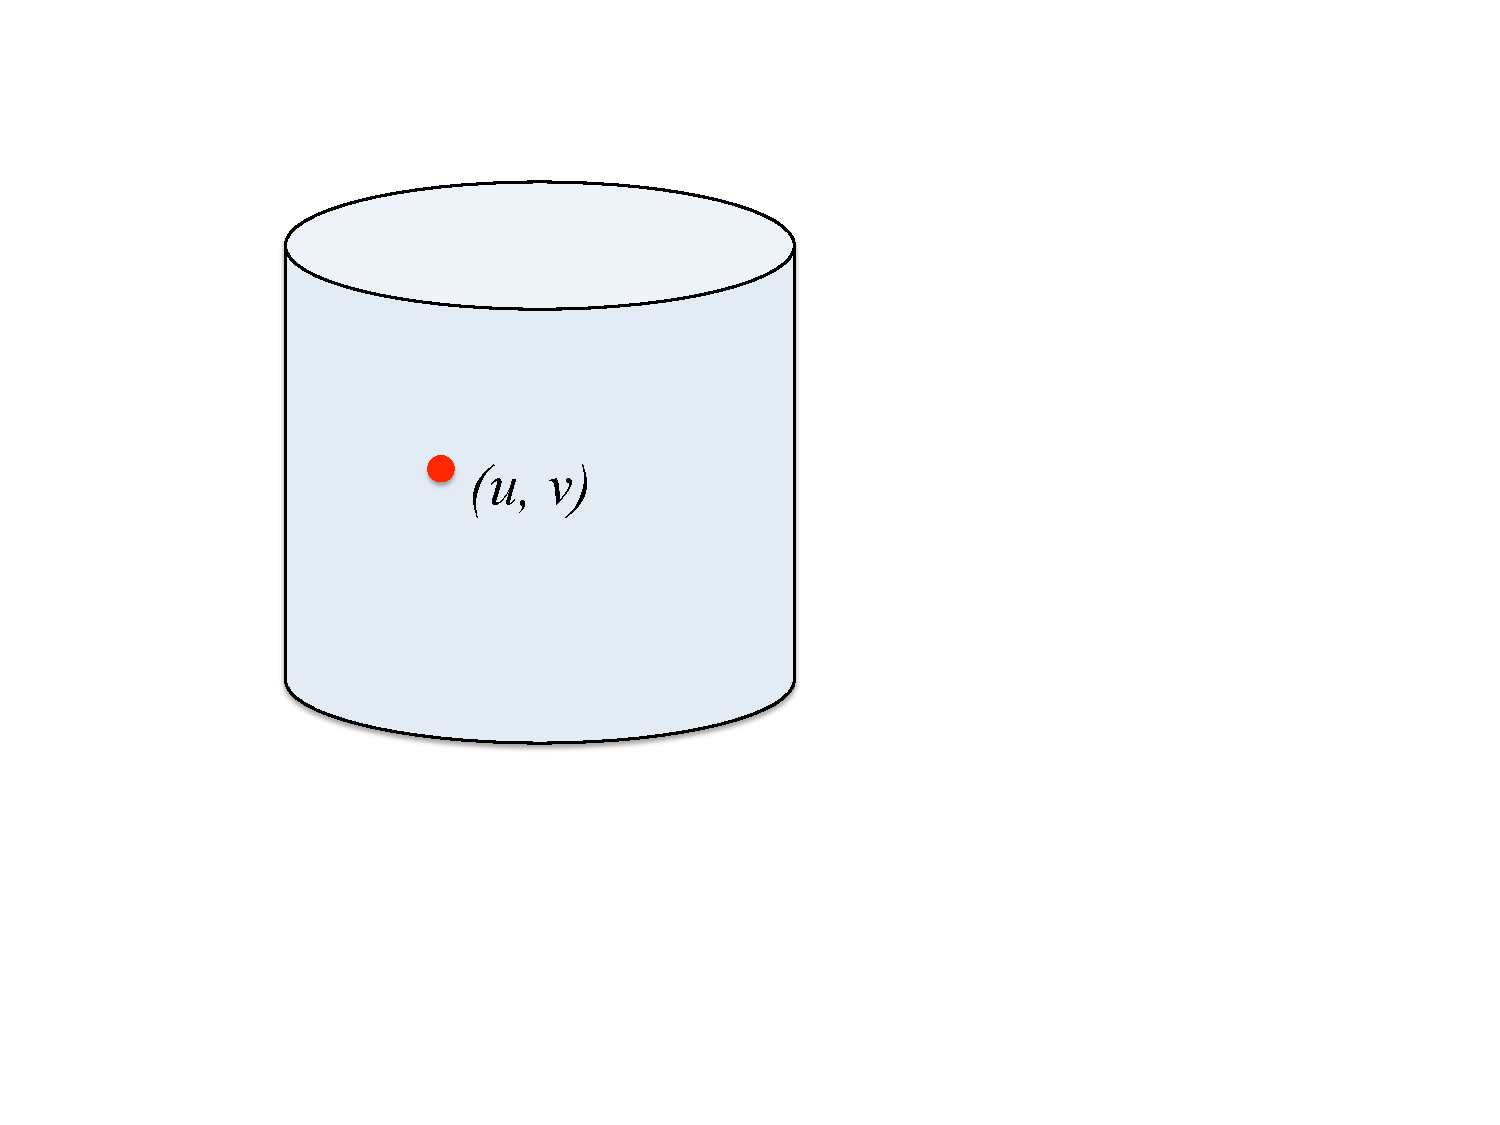
\includegraphics[width=\subwidth, clip=true, trim=130 105 300 30]{features_2}}
\begin{figure}
%     %\subfigure[]{%
     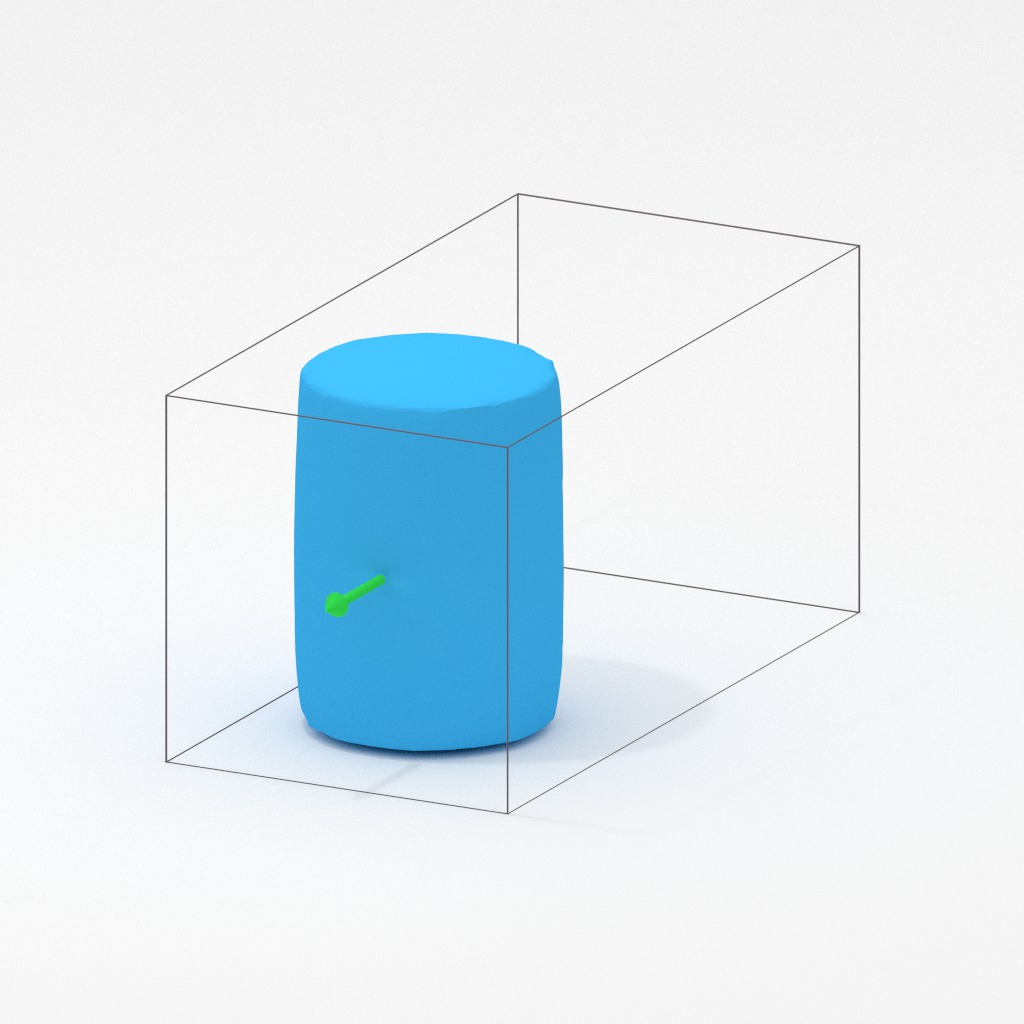
\includegraphics[width=0.3\columnwidth]{voxlets/1_marching_cubes}
     \includegraphics[width=0.3\columnwidth]{voxlets/5_marching_cubes}
     \includegraphics[width=0.3\columnwidth]{voxlets/10_marching_cubes} \\
     \includegraphics[width=0.3\columnwidth]{voxlets/19_marching_cubes}
     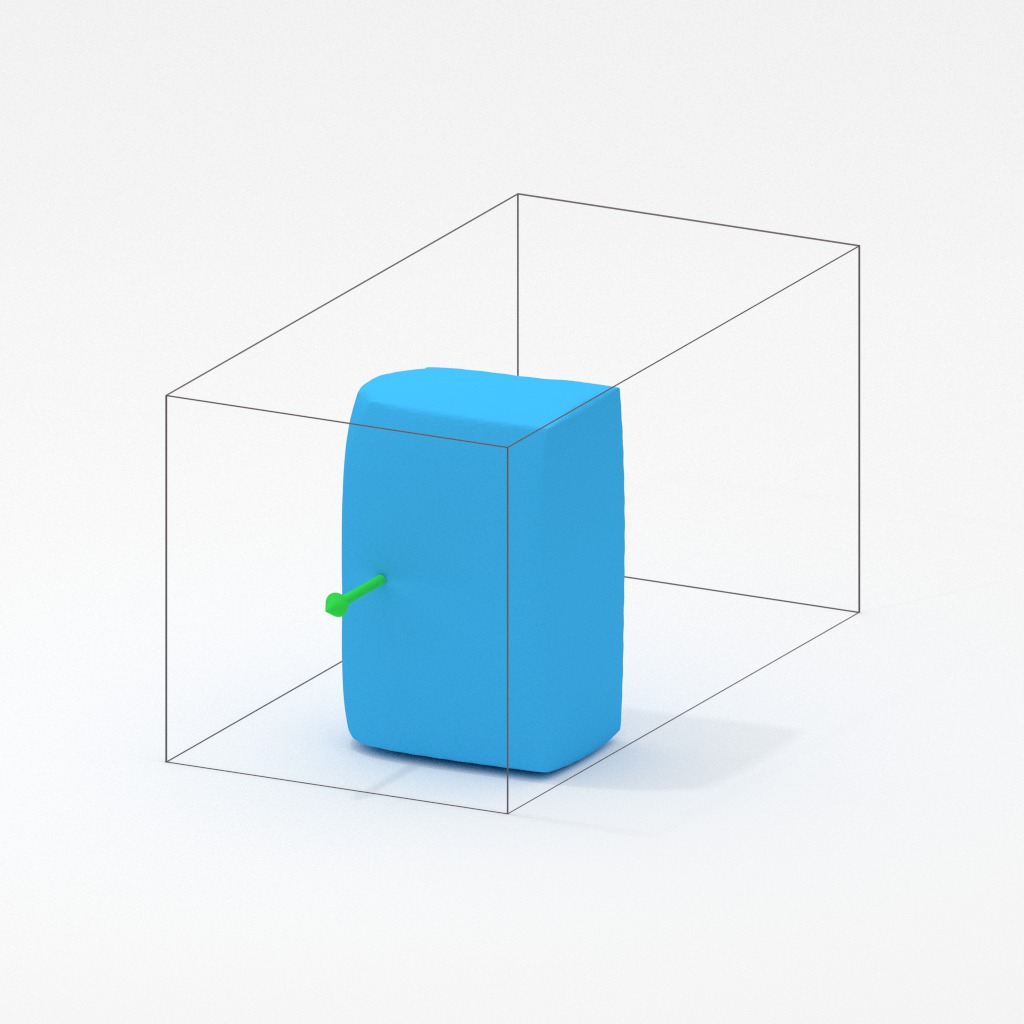
\includegraphics[width=0.3\columnwidth]{voxlets/38_marching_cubes}
     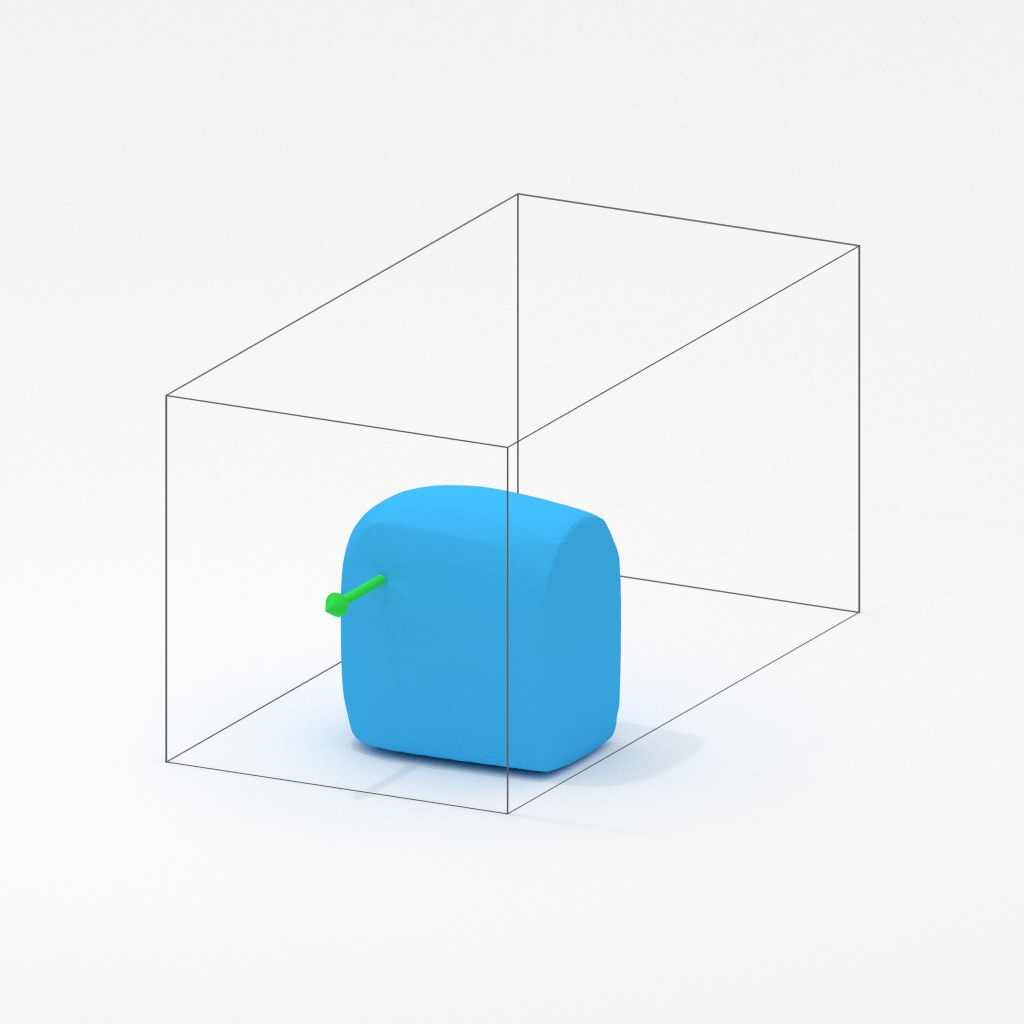
\includegraphics[width=0.3\columnwidth]{voxlets/44_marching_cubes}
     \caption{Some of the voxlets detected from the Bigbird dataset}
\end{figure}
%     %}
%     % \subfigure[]{%
%     % \includegraphics[width=\voxletsubwidth, clip=true, trim=\voxcropl \voxcropbot \voxcropr \voxcropr]{5_marching_cubes}
%     % }
%     % \subfigure[]{%
%     % 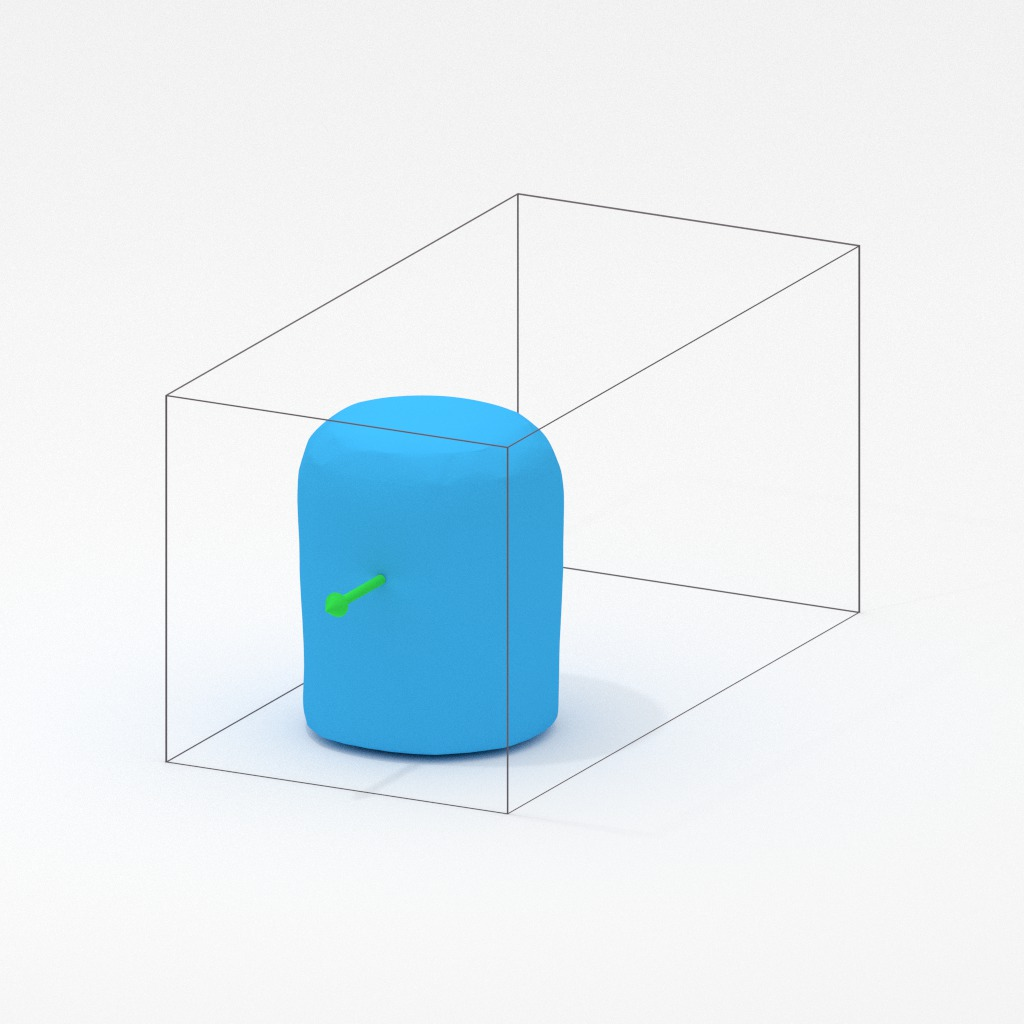
\includegraphics[width=\voxletsubwidth, clip=true, trim=\voxcropl \voxcropbot \voxcropr \voxcropr]{8_marching_cubes}
%     % }
%     % \subfigure[]{%
%     % \includegraphics[width=\voxletsubwidth, clip=true, trim=\voxcropl \voxcropbot \voxcropr \voxcropr]{10_marching_cubes}
%     % }
%     % \subfigure[]{%
%     % \includegraphics[width=\voxletsubwidth, clip=true, trim=\voxcropl \voxcropbot \voxcropr \voxcropr]{19_marching_cubes}
%     % }
%     % \subfigure[]{%
%     % 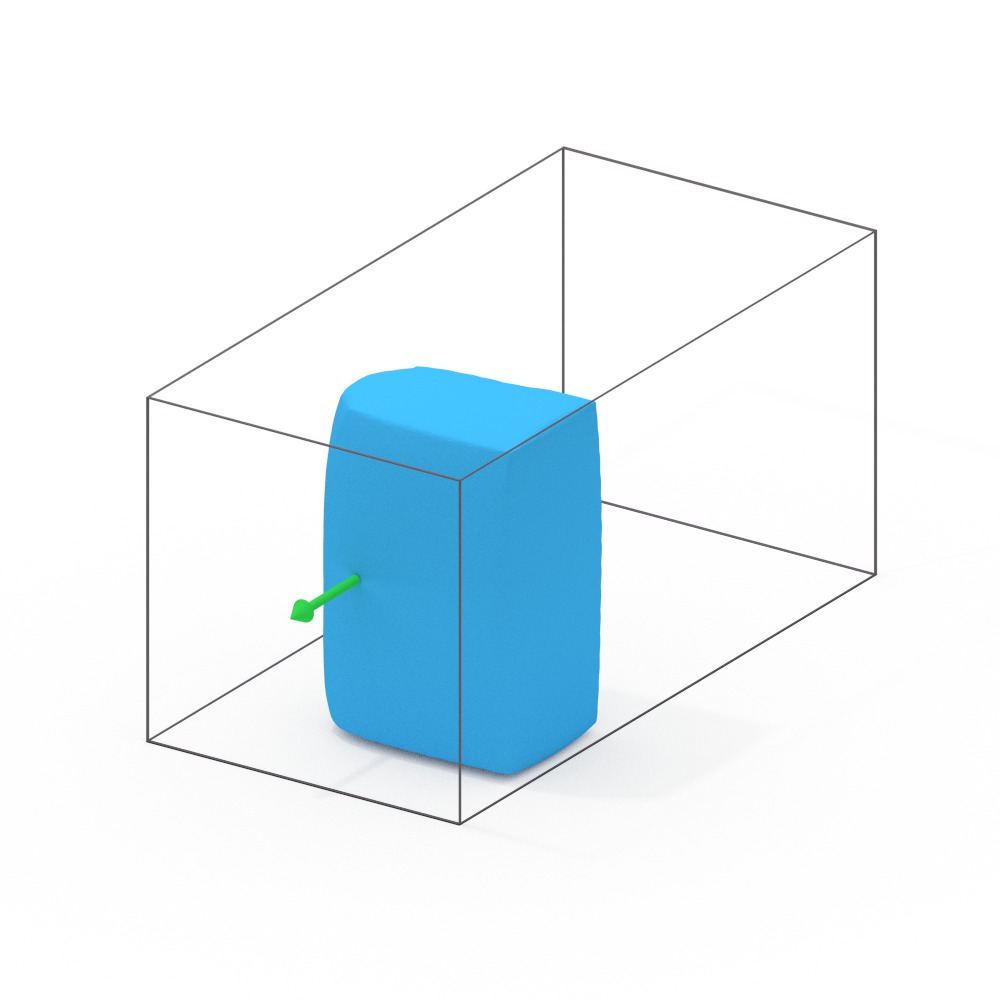
\includegraphics[width=\voxletsubwidth, clip=true, trim=\voxcropl \voxcropbot \voxcropr \voxcropr]{38_marching_cubes}
%     % }
%     % \subfigure[]{%
%     % 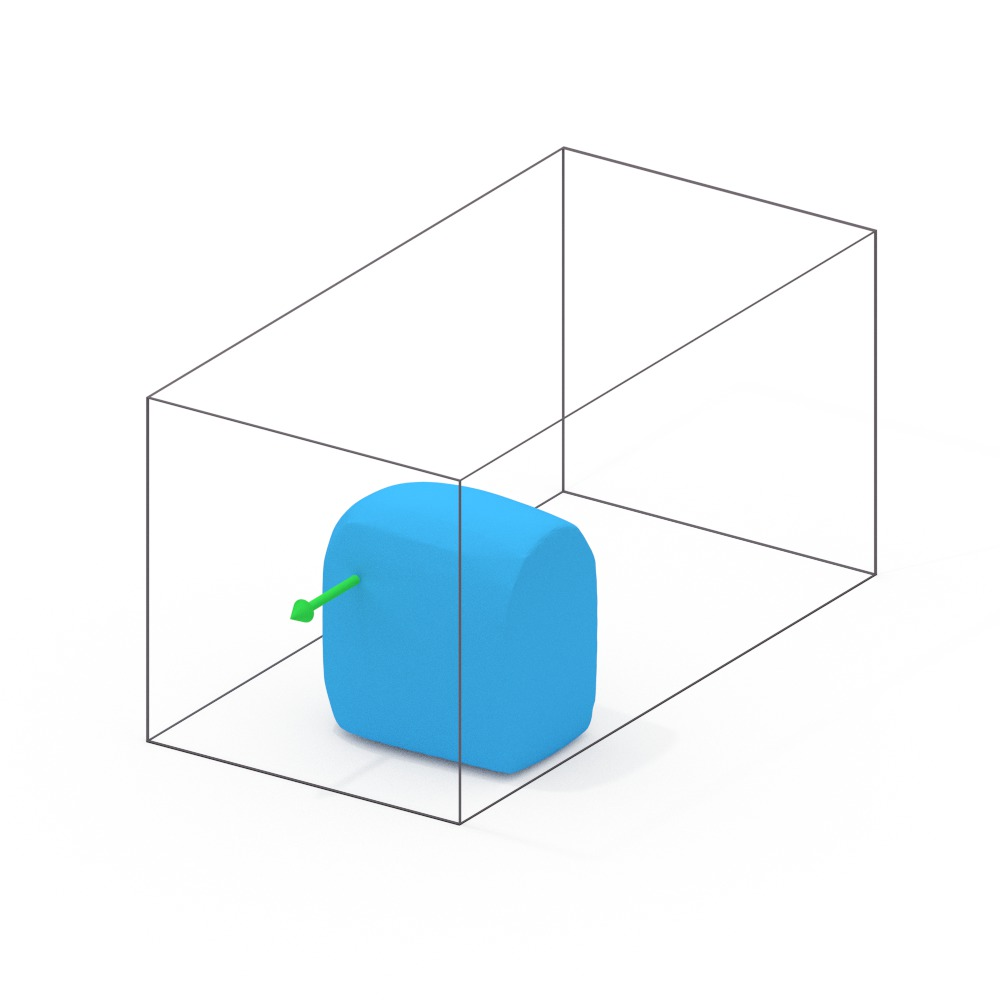
\includegraphics[width=\voxletsubwidth, clip=true, trim=\voxcropl \voxcropbot \voxcropr \voxcropr]{44_marching_cubes}
%     % }
%     \caption{
%     Some of the voxlets extracted from the Bigbird dataset.
%     }%
%     \label{fig:voxlets}





\newcommand{\preprocesssubwidth}{0.41\columnwidth}
\begin{figure*}[tb]
    \centering 
    \subfigure[RGB image]{%
        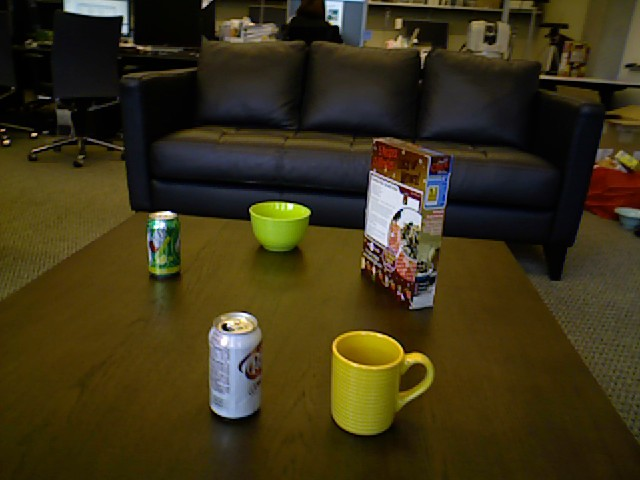
\includegraphics[width=\preprocesssubwidth]{preprocess_a}}
        \hfill
    \subfigure[Raw depth image]{%
        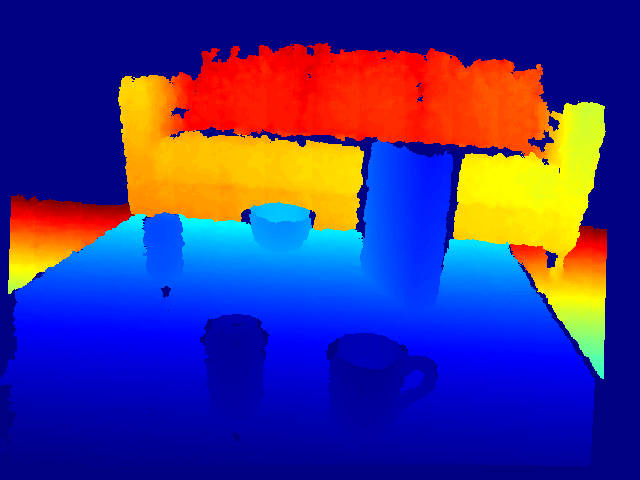
\includegraphics[width=\preprocesssubwidth]{preprocess_b}}
        \hfill
    \subfigure[Smoothed depth]{%
        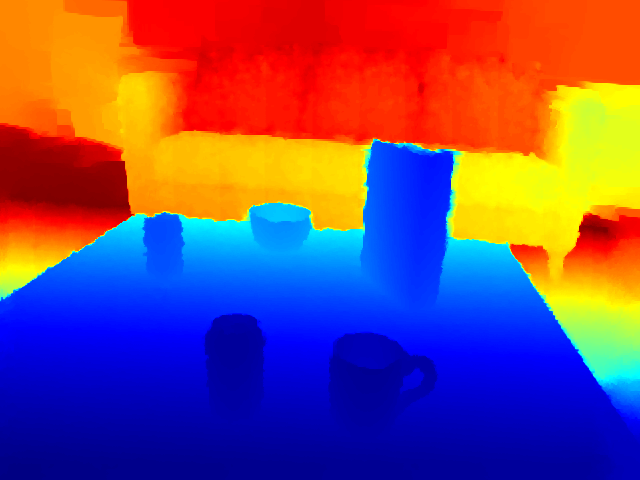
\includegraphics[width=\preprocesssubwidth]{preprocess_c}}
        \hfill
    \subfigure[Structured edges]{%
        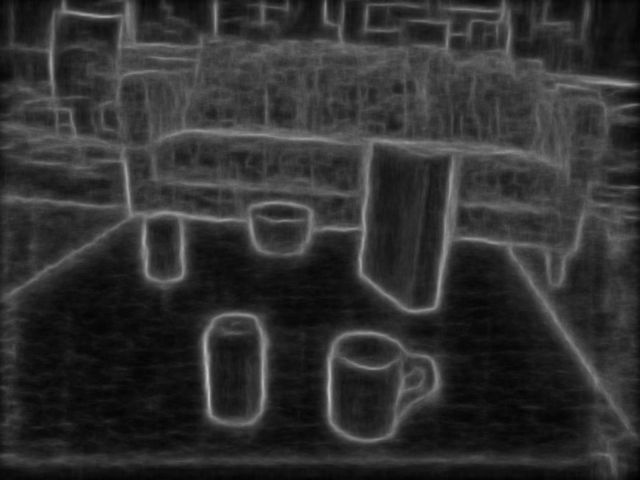
\includegraphics[width=\preprocesssubwidth]{preprocess_d}\label{subfig:structedge}}
        \hfill
    \subfigure[Binary edge map]{%
        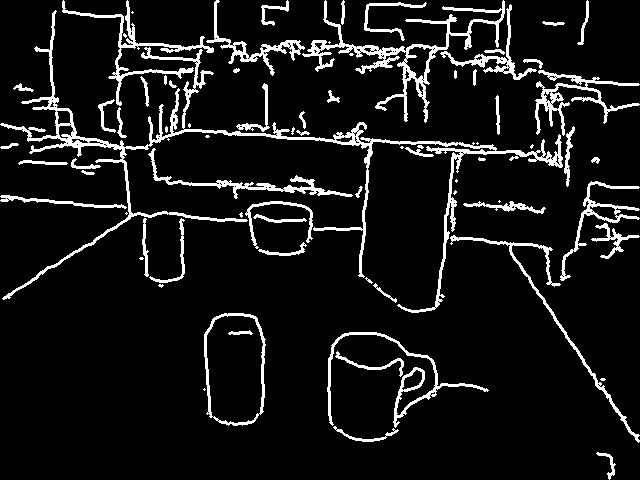
\includegraphics[width=\preprocesssubwidth]{preprocess_e}\label{subfig:binaryedge}}
    \caption{
    Preprocessing
    }%
    \label{fig:preprocessing}
\end{figure*}


%%%%%%%%%%%%%%%%%%%%%%%%%%%%%%%%%%%%%%%%%%%%%%%%%%%%%%%%%%%%%%%%%%%%%%%%%%%%%%%%%
\section{Feature representation}
%%%%%%%%%%%%%%%%%%%%%%%%%%%%%%%%%%%%%%%%%%%%%%%%%%%%%%%%%%%%%%%%%%%%%%%%%%%%%%%%%

We use local and regional features extracted from the image around $\pixelidx$ to represent the geometry around the point.
This is used in our classifier to map from a single point to a prediction of voxel occupancy in the surrounding region.

We use two novel features. 
The \emph{cobweb} feature captures the shape of the depth surface in the immediate vicinity of $\pixelidx$. 
The \emph{spider} feature captures the size and shape of the region in which $\pixelidx$ resides together with the position of $\pixelidx$ in that region\footnote{The names of our features are taken from the shapes they produce in image space (figure \ref{fig:features}).}.


%%%%%%%%%%%%%%%%%%%%%%%%%%%%%%%%%%%%%%%%%%
\subsubsection{Cobweb feature }
%\note{Name up for debate!}
The cobweb feature is a simple pairwise feature, related to recent work such as \cite{shotton-cvpr-2011, tola-pami-2010}, capturing the surface shape in the immediate vicinity of pixel $\pixelidx$.
The feature computes the difference between the depth from the camera at $\pixelidx$ and the depth at a predetermined offset.
\begin{align}
\Phi_c(u, v, \psi, t) &= \rgbdimage(u, v) - \rgbdimage(a, b) \\
a &= \left\lfloor u + M(t)  \sin(\psi) \right\rceil \\
b &= \left\lfloor v + M(t)  \cos(\psi) \right\rceil
\end{align}
where $M(t) = ft / \rgbdimage(\pixelidx)$ uses the focal length $f$ to map a distance in world space to a pixel offset. For our experiments we compute the cobweb feature for all combinations of $\psi = [0\degree, 45\degree, \ldots, 315\degree]$ and $t = [0.02m, 0.04m, 0.06m]$.
The final cobweb feature is therefore 24-dimensional.
%Note also: ``If an offset pixel lies on the background or outside the bounds of the image, the depth probe dI (x0) is given a large positive constant value''.

%%%%%%%%%%%%%%%%%%%%%%%%%%%%%%%%%%%%%%%%%%
\subsubsection{The spider feature}
%\note{Name up for debate! Another candidate is `compass'}

Local features such as our cobweb feature have proved discriminatory where the output labeling is on a per-pixel basis, such as labeling each pixel as a part of a human body \cite{shotton-cvpr-2011}.

However, when it comes to predicting the geometry of the scene we cannot observe, the local shape of the depth image around a point does not provide enough information. 
An example of this can be seen in figure \ref{fig:patch_problems}.
The two regions circled in the image have identical \emph{local} appearance, but the 3D geometry around each regions is very different due to the different thicknesses of the two boxes.


\begin{figure}[bt]
  \centering 
  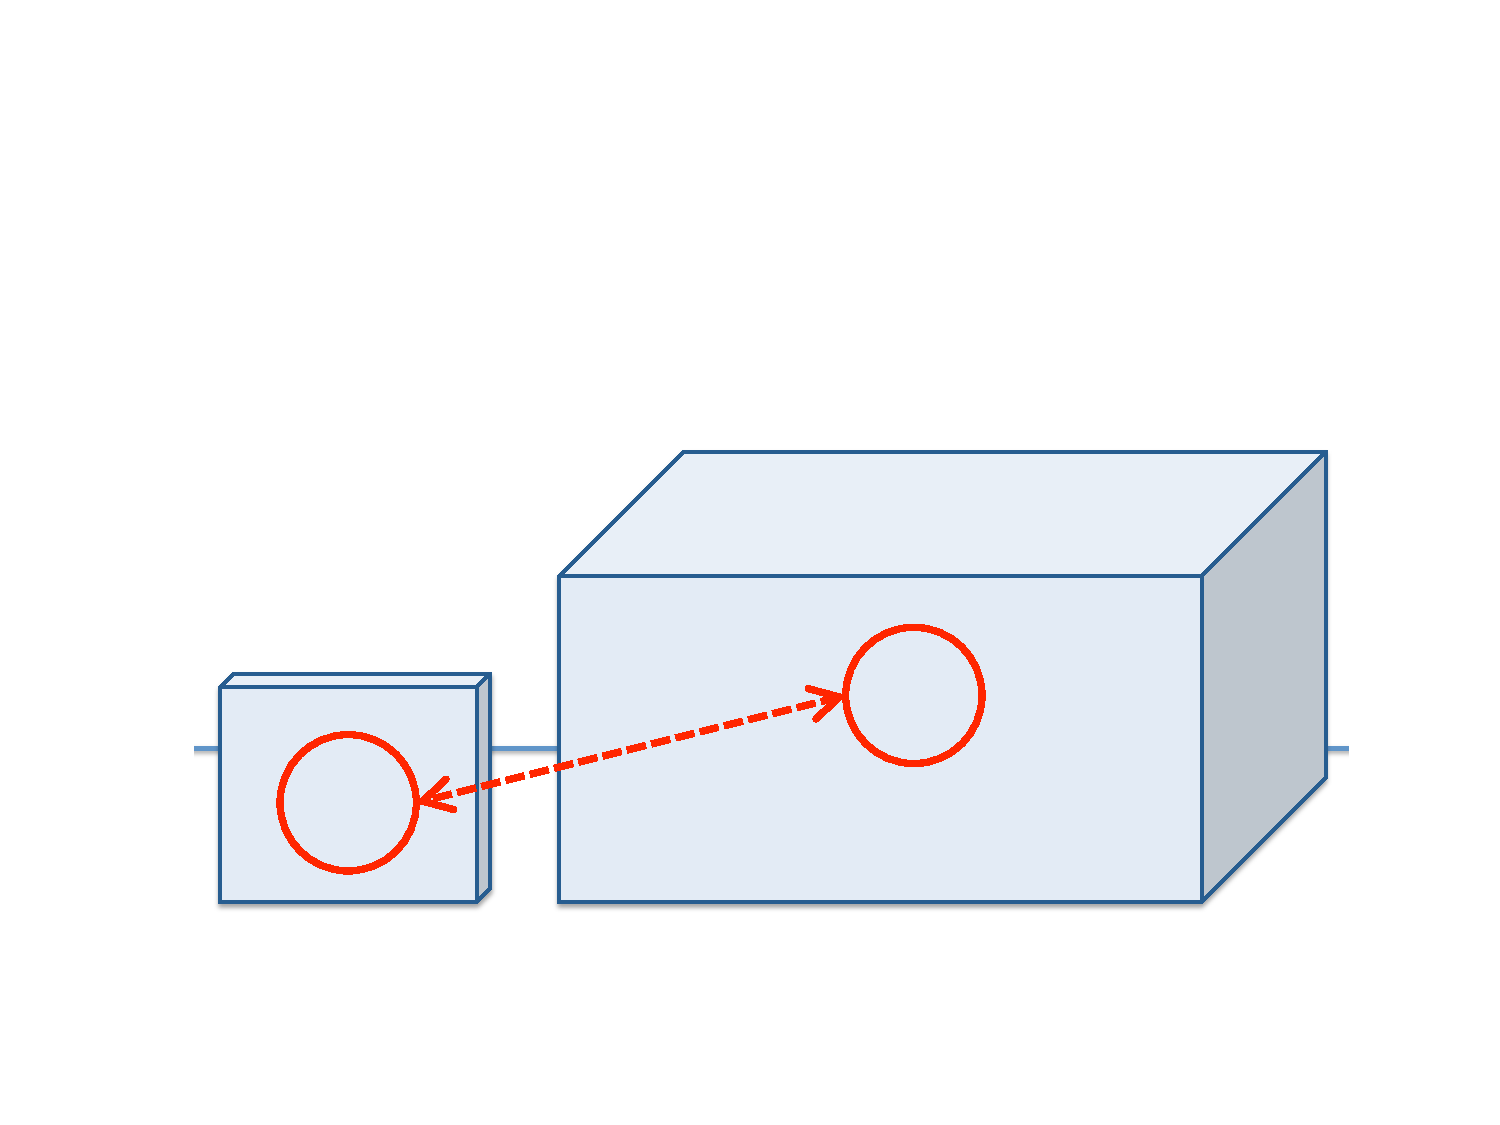
\includegraphics[width=0.9\columnwidth]{features_1}
  \caption{Local, patch-type features do not give enough information to accurately predict depth. Here, a pair of regions on two different objects are marked. Each region has identical local appearance. However, the thickness of the object at the two locations is very different. 
  We use this observation to motivate the spider feature.}
  \label{fig:patch_problems}
\end{figure}
%\todo{Combine all the motivational images for the spider feature into one...}}


Previous works have used the properties of a whole segmented region for classification of individual points \cite{golovinskiy-iccv-2009}.
When it comes to predicting the 3D shape local to a point in an image, however, we care as much about the point's location in the region as we do about the overall region properties (figure \ref{fig:spider_motivation}).

We desire a feature which captures the size and shape of the region in which $\pixelidx$ resides, along with the location of $\pixelidx$ in that region.
To achieve this we take inspiration from the features between a point and a binary edge map used by \cite{drost-3dimpvt-2012}.

\paragraph{Computing a binary edge map}
We first compute a binary edge map for the image, where each pixel takes the value 1 at a large change in depth or surface normal direction, and is 0 otherwise.
We first use the method of \cite{dollar-iccv-2013} to compute a real-valued edge map for the image (figure \ref{subfig:structedge}).
Next we apply the Canny filtering algorithm \cite{} to convert this to a binary edge map (figure \ref{subfig:structedge}).
We mitigate against poor quality depth data around discontinuities by dilating this edge map with a 3x3 disc-shaped structuring element.

\paragraph{Casting lines from $\pixelidx$}
From $\pixelidx$, we then cast a line across the edge map in direction $\phi$.
We note the point on the edge map where the line first hits a pixel with value 1 as $\edgeimidx$.
The 2D locations $\pixelidx$ and $\edgeimidx$ reproject to 3D locations $\project(\pixelidx)$ and $\project(\edgeimidx)$ respectively.
%For each line cast we therefore have two points in 3D space: $\point$ and $\point_e$.



\newcommand{\subwidth}{0.32\columnwidth}
\begin{figure*}[tb]
    \centering 
    \subfigure[Query point]{%
        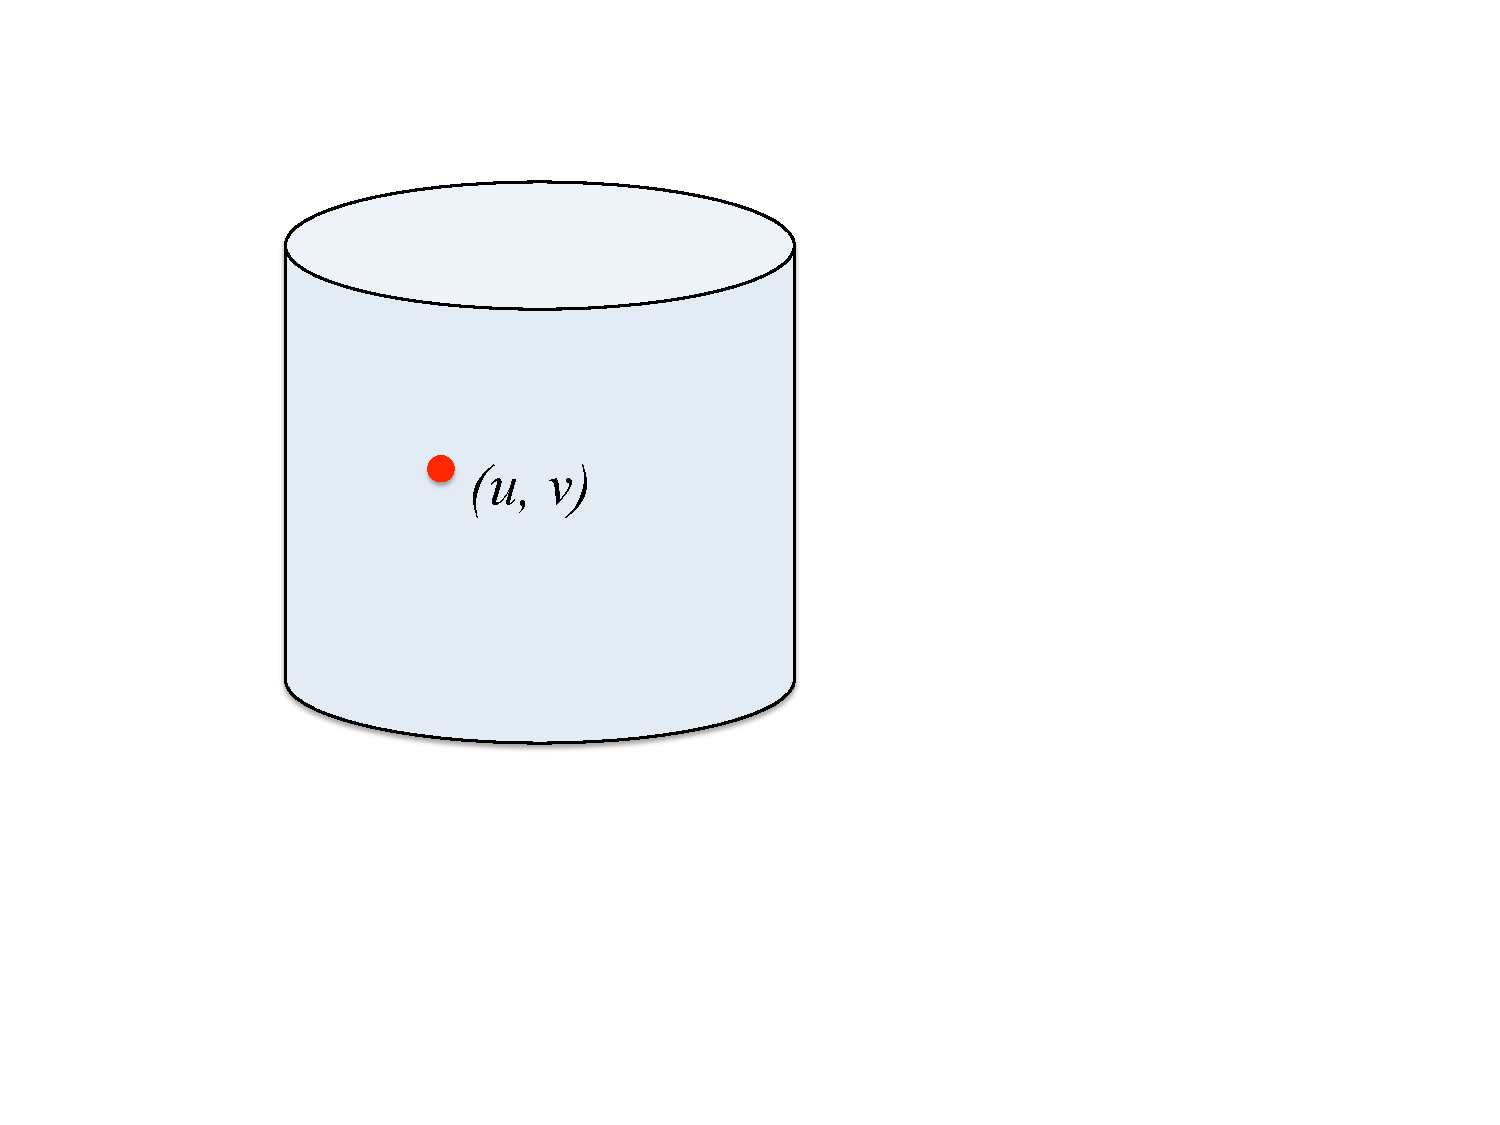
\includegraphics[width=\subwidth, clip=true, trim=130 105 300 30]{features_2}}
        \hfill
    \subfigure[Cobweb feature]{%
        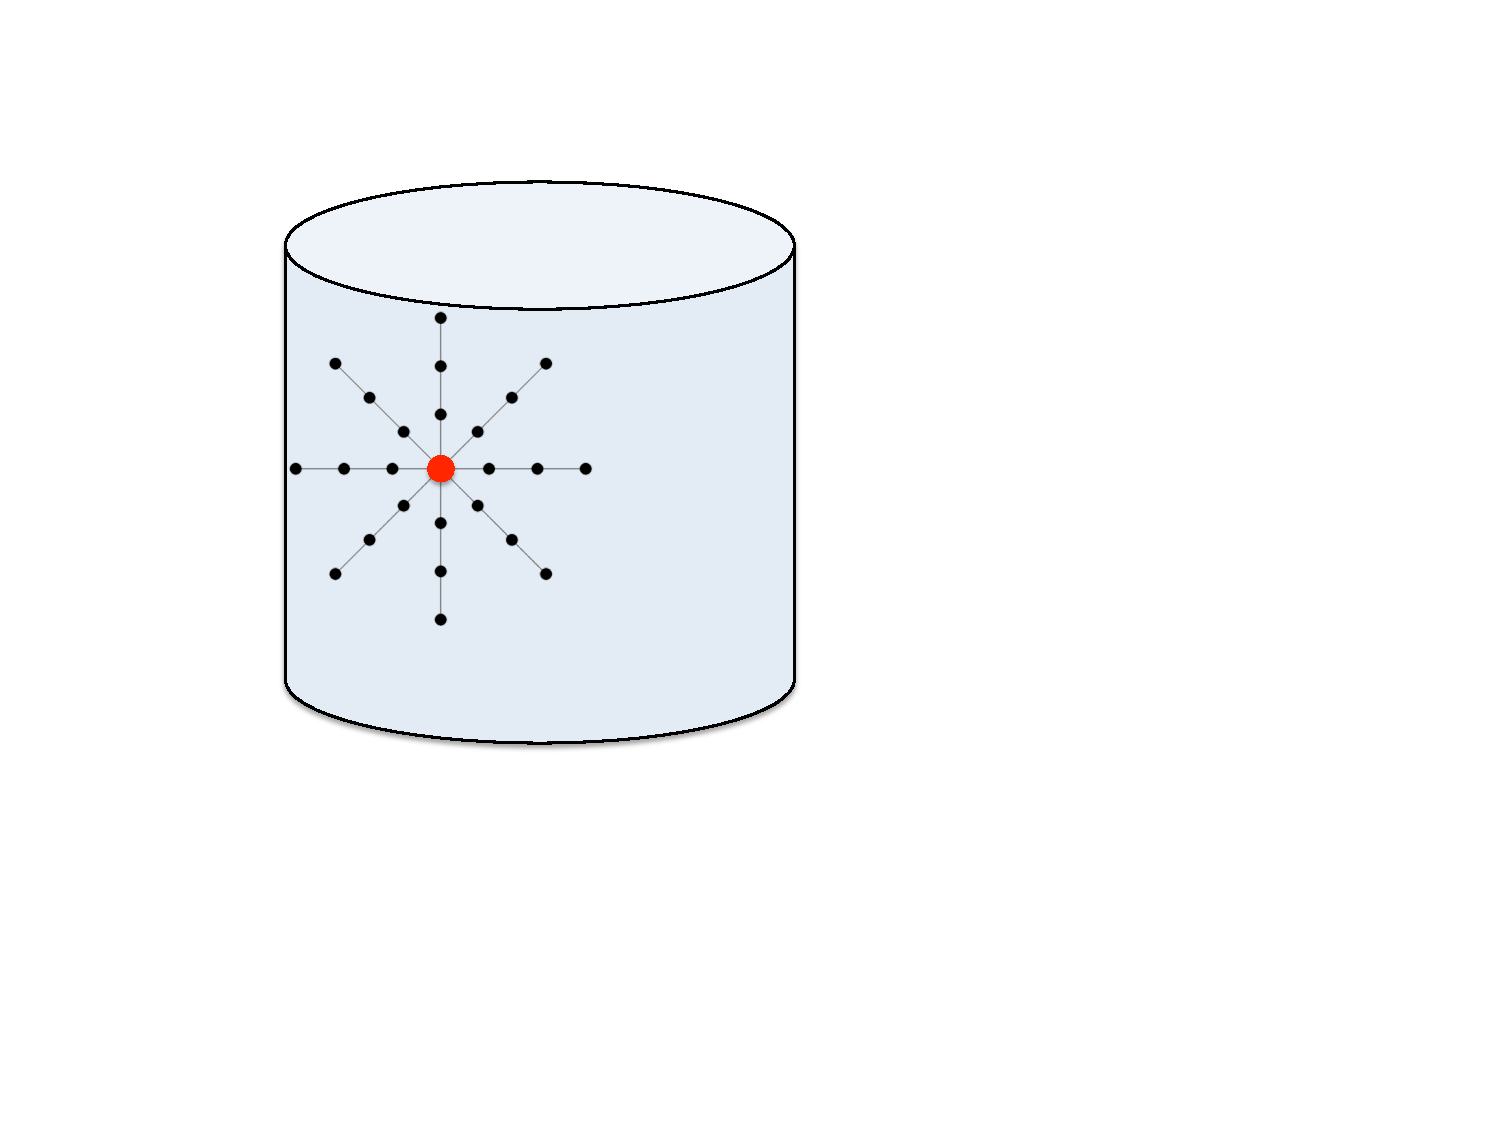
\includegraphics[width=\subwidth, clip=true, trim=130 105 300 30]{features_3}
        \label{fig:features:occluded_spider}}
        \hfill
    \subfigure[Spider feature]{%
        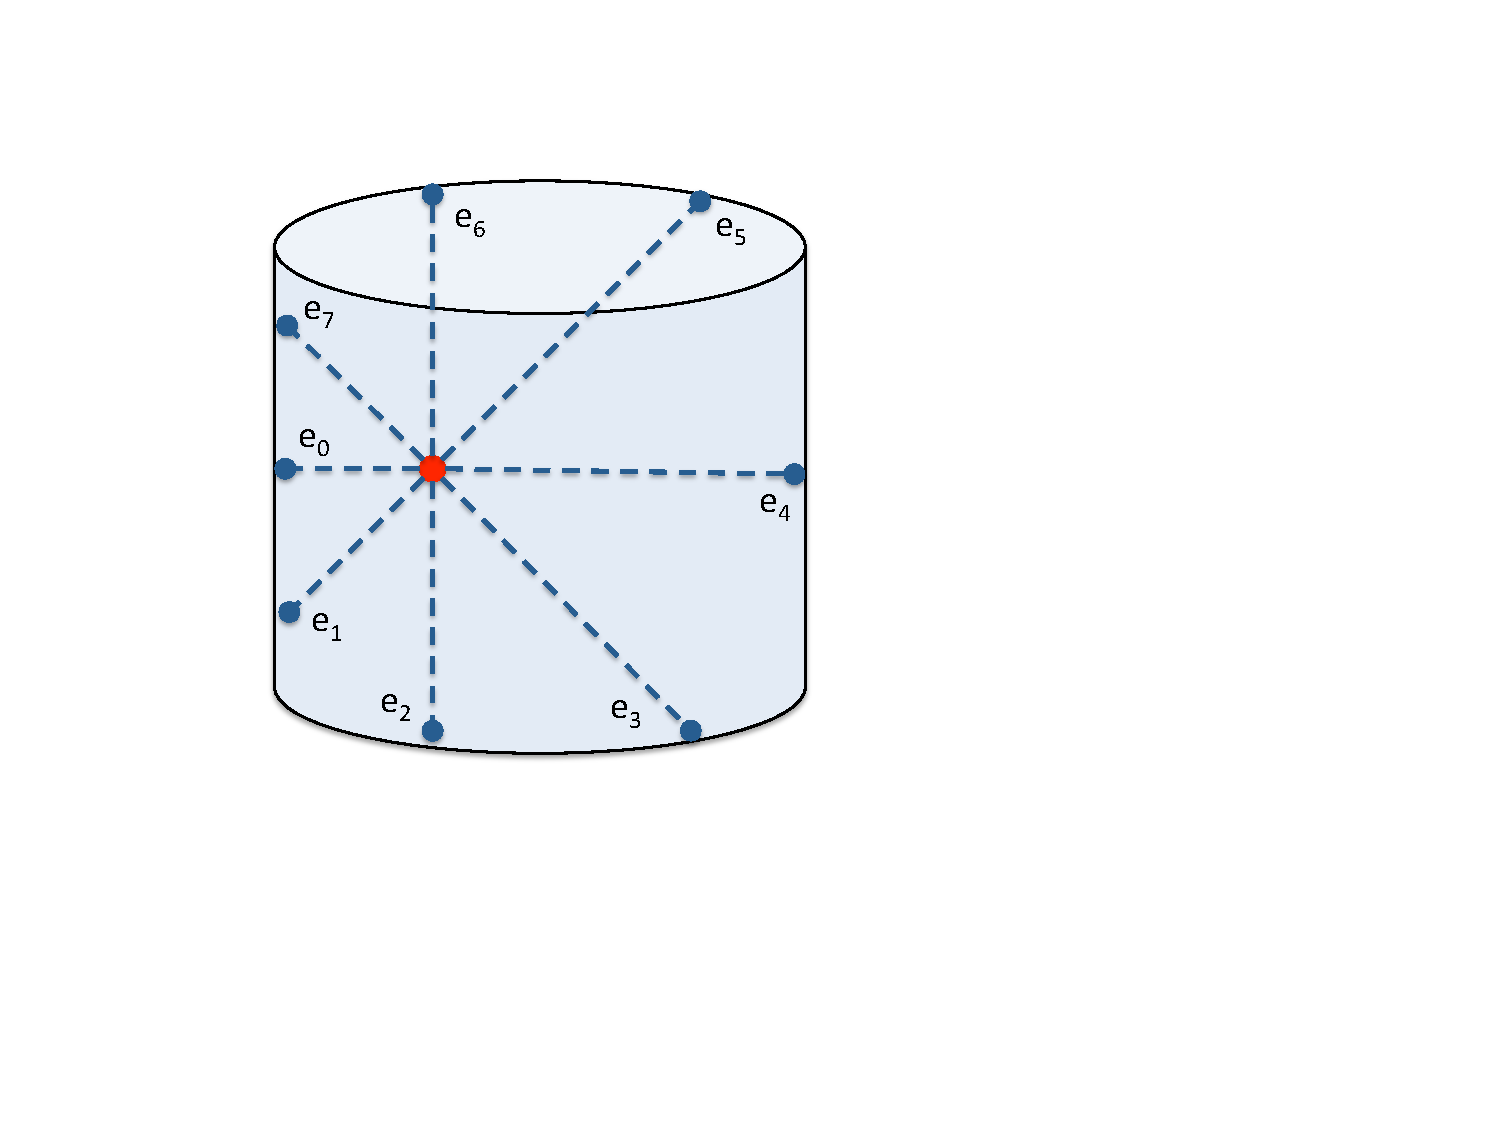
\includegraphics[width=\subwidth, clip=true, trim=130 105 300 30]{features_4}}
        \hfill
    \subfigure[$c_0$]{%
        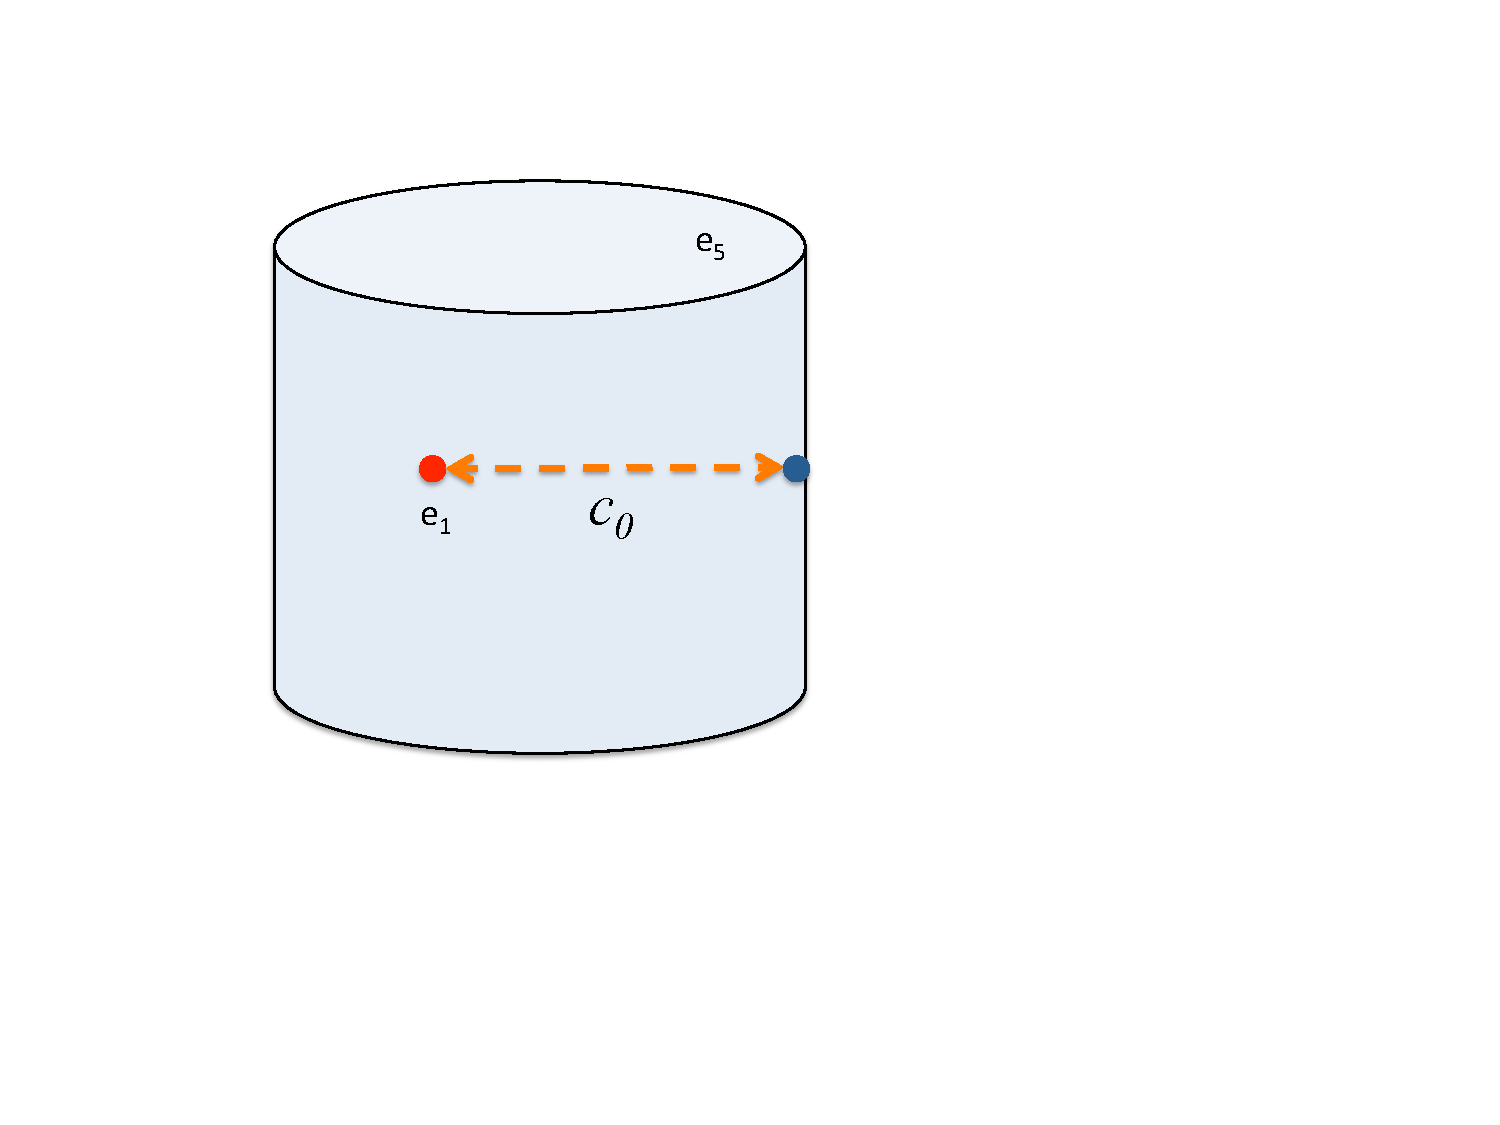
\includegraphics[width=\subwidth, clip=true, trim=130 105 300 30]{features_5}\label{subfig:c0}}
        \hfill
    \subfigure[$c_1$ (Top view of scene)]{%
        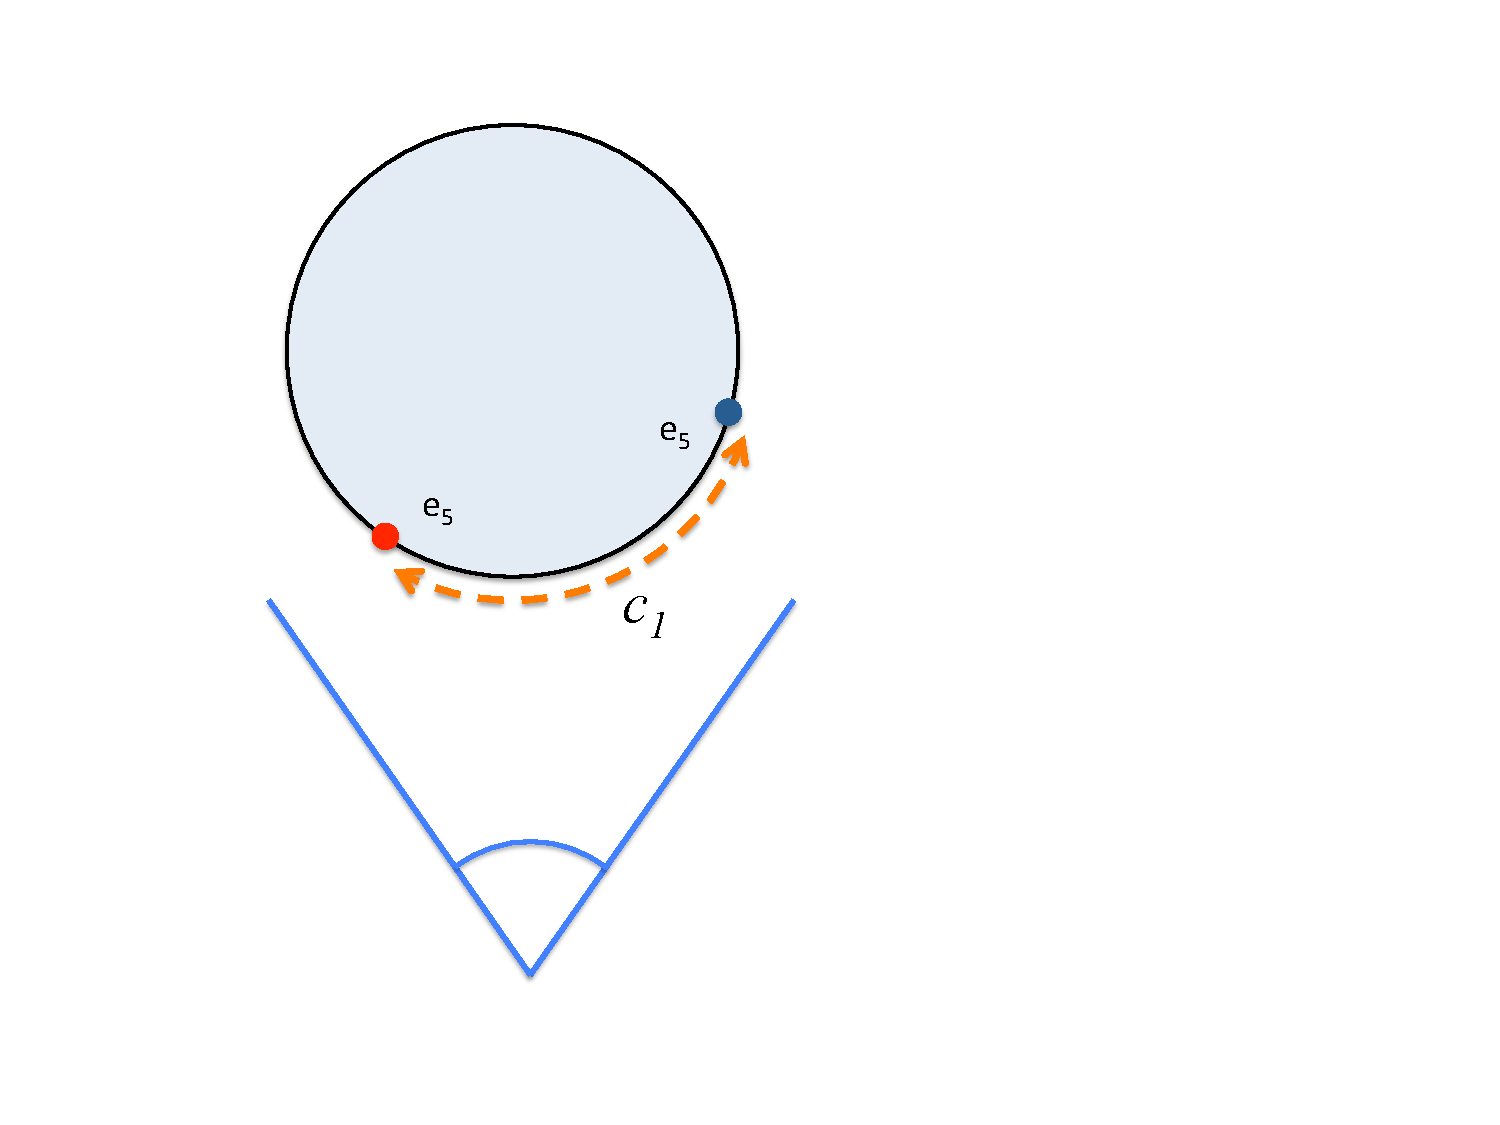
\includegraphics[width=\subwidth, clip=true, trim=130 70 300 30]{features_6}\label{subfig:c1}}
        \hfill
    \subfigure[$c_2$ (Top view of scene)]{%
        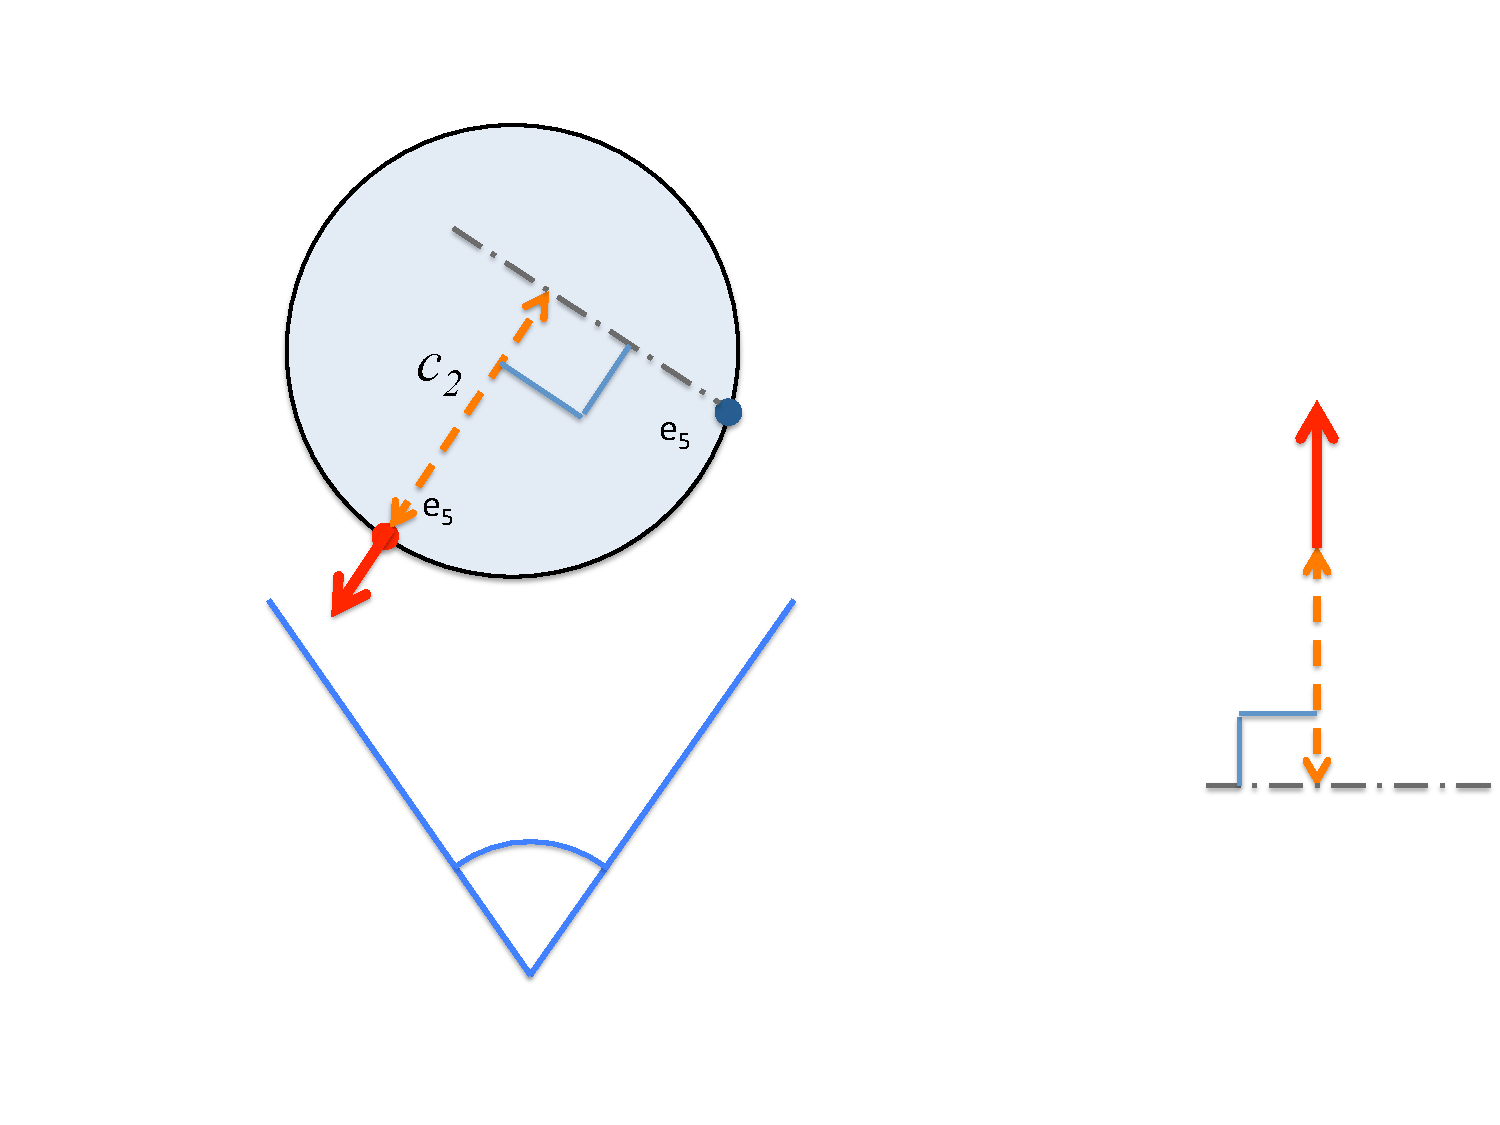
\includegraphics[width=\subwidth, clip=true, trim=130 70 300 30]{features_7}\label{subfig:c2}}
        \hfill
    \caption{
    %(a) Each point on a depth image has an angle $\theta$ associated, which represents the direction of gradient of the depth. 
    (b) The spider features measure the distance between $\point$ and the edge points $e_{1, \cdots, 7}$.
    %(c) Because the spider features are computed relative to $\theta$, the resultant feature vector is invariant to object rotations in the camera plane.
    (d) Where the spider line emitted from $\point$ first hits an occluded edge, only a \textit{minimum} extent is known.
    This case is denoted as \texttt{?} in this figure.
    (e) The cobweb feature measures the difference in depth between $\point$ and a set of points in the near vicinity of $\point$, arranged in a cobweb shape.}%
    \label{fig:features}
\end{figure*}



\paragraph{Extracting the spider feature}

\newcommand{\spiderfeat}{s}

The spider feature for a single point with a line cast in direction $\phi$ is $\Phi_s = (\spiderfeat_0, \spiderfeat_1, \spiderfeat_2)$.
Each element of this tuple is completed as follows:
\begin{itemize}

\item $\spiderfeat_1 = \rgbdimage(\pixelidx) \|\pixelidx - \edgeimidx\| / f$. This is the distance between $\pixelidx$ and $\edgeimidx$ in pixel units $\|\pixelidx - \edgeimidx\|$ scaled by $\rgbdimage(\pixelidx) / f$ to convert to a real-world distance (figure \ref{subfig:c0}).

\item $\spiderfeat_2 = (\point(\pixelidx) - \point(\edgeimidx)) \cdot \normal$. 
This is the Euclidean distance between $\point(\pixelidx)$ and $\point(\edgeimidx)$ along the direction of the normal at $\pixelidx$  (figure \ref{subfig:c1}).

\item $\spiderfeat_3 = \sum_{i=2}^{|l|} \| \project(l_i) - \project(l_{i-1}) \| $, where $l$ is an ordered list of the pixel locations on the line between $\pixelidx$ and $\edgeimidx$.
This is the arc length between $\pixelidx$ and $\edgeimidx$ along the surface of $\rgbdimage$  (figure \ref{subfig:c2}).
\end{itemize}

%\item the \textbf{geodesic distance} $d_g(\point, point_e)$ across the surface of $\rgbdimage$

We compute the spider features for  $\phi = [0\degree, 45\degree, \ldots, 315\degree]$
The spider feature for a single point $\pixelidx$ is therefore 16-dimensional.

\paragraph{Implementation}
The spider feature is extremely efficient to compute.
This is due to its cumulative nature: $(u, v, 0)$ can be directly computed from $s(u, v-1, 0)$.
We can compute the 16D spider feature for every point in a $640\times480$ image in less than 0.01s using unoptimized C++ code.
We would expect a significant speedup were this to be implemented on a GPU.


\paragraph{Occluded spider features}

We explicitly handle occlusion in the spider features. Where the spider feature first hits an occluded edge rather than an occluding edge, the true size of the object in that dimension is unknown (see figure \ref{fig:features:occluded_spider}).
However, we do have a \textit{minimum} size in that direction.

We reason that discontinuities in depth images can be assigned a direction: one side of each edge is the occluder, the other is the occludee. 
We can compute the gradient of the depth edges using PCA on the edge pixels in image space.
We ensure that the final gradient at each edge pixel points in the direction of the occluded side.

We can then use the occlusion information in our feature computations.
See for example figure \ref{fig:occluded_region}.

Motivation:
\begin{itemize}
\item Local features not good for many purposes (image)
\item Region features capture properties of region (image)
\item BUT We want to know where we are in a region  (image)
\item Also the properties of a region can change over space (image)
\item Occluded regions
\end{itemize}




% \begin{figure}
%     \centering 
%     \subfigure[]{%
%         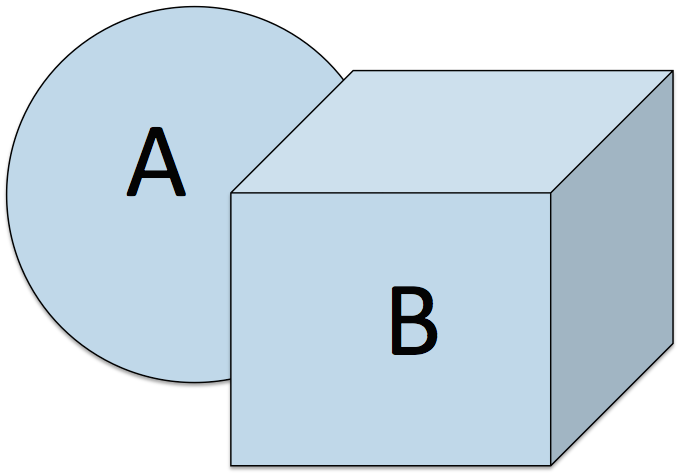
\includegraphics[width=0.45\columnwidth]{occlusion_a}}
%         \hfill
%     \subfigure[]{%
%         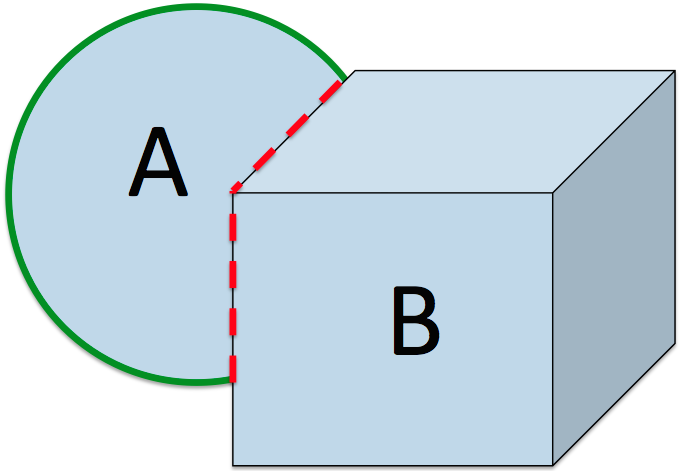
\includegraphics[width=0.45\columnwidth]{occlusion_b}} \\
%     \caption{Where edges occur as a result of occlusion boundaries, the direction of the edge is important. The edge bounding region A can be divided into an \emph{occluding} portion (solid green) and an \emph{occluded} portion (dashed red).
%     We can make a reasonable assumption that region A may extend behind object B past the occluded edge.
%     However, region A cannot continue sideways beyond its occluding edge.}
%     \label{fig:occluded_region}
% \end{figure}

% \begin{figure}
%     \centering% 
%     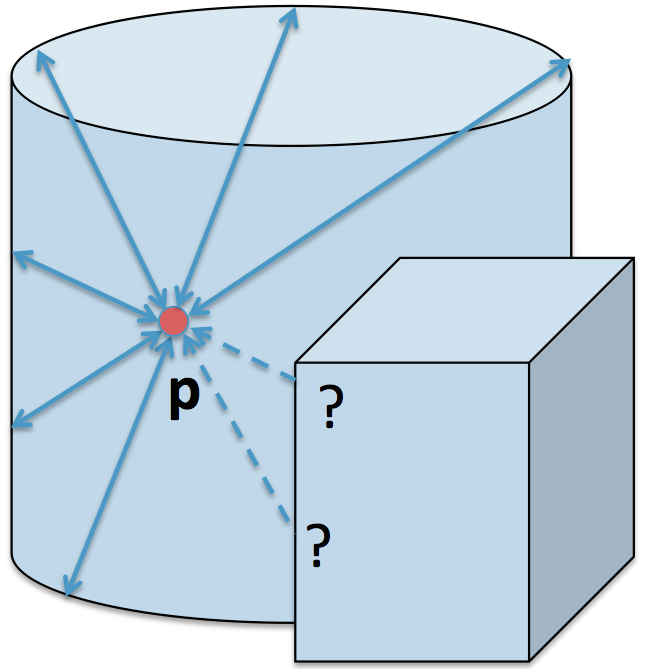
\includegraphics[width=0.7\columnwidth]{occlusion_spider.png}% 
%     \figcaption{The spider feature extends lines from $\point$ to the first occluding edge found along the path. Internal edges (e.g. those found in RGB space) are ignored. Where the line first hits an occluded edge, the true extent is unknown --- this case is denoted as \texttt{?} in this figure.}% 
%     \label{fig:occluded_spider}% 
% \end{figure}


% %%%%%%%%%%%%%%%%%%%%%%%%%%%%%%%%%%%%%%%%%%%%%%%%%%%%%%%%%%%%%%%%%%%%%%%%%%%%%%%%
\section{Learning a mapping from features to voxlets}
% %%%%%%%%%%%%%%%%%%%%%%%%%%%%%%%%%%%%%%%%%%%%%%%%%%%%%%%%%%%%%%%%%%%%%%%%%%%%%%%%


A Random Forest is a set of decision trees, each of which is trained on a different subset of the training data \cite{breiman-ml-2001}.
At test time, each data point is passed through each tree, and at each node is passed left or right depending on the feature thresholds learned at training time. The final leaf node the data point ends in will vote for a class, based on which training samples ended up at that leaf node.

Random Forests are well suited to our purpose, as they automatically select the features most suitable for separating the classes (unlike \eg SVMs) and they examine each dimension separately, making them robust to different scaling of each feature. They are also inherently non-linear, perform quick training and inference and are easily parallelizable.

%In our case, the classes correspond to $y_{ij}$ and $\lnot y_{ij}$, which we now refer to as $y^{+}$ and $y^{-}$ for ease of notation.

%\subsection{Training the forest}
In training our forest we use the entropy split criterion
\begin{equation}
- \sum_j p_j \log_2 p_j.
\end{equation}
at each node.

Often the modal class vote from all the trees is taken as a hard prediction of class membership. Instead we follow \cite{} in using... medioid? Modal?

% \cite{bostrom-mla-2007} in using the fraction of votes for each class to approximate a probability of class membership. $p_{ij}$ can be interpreted as the parameter of a categorical distribution.





% %%%%%%%%%%%%%%%%%%%%%%%%%%%%%%%%%%%%%%%%%%%%%%%%%%%%%%%%%%%%%%%%%%%%%%%%%%%%%%%%
\section{Notes}
% %%%%%%%%%%%%%%%%%%%%%%%%%%%%%%%%%%%%%%%%%%%%%%%%%%%%%%%%%%%%%%%%%%%%%%%%%%%%%%%%
Just some notes of things to also include:

\begin{itemize}
\item Literature on surface descriptions (normal estimation? depth/sliding window?)
\begin{itemize}
\item Patch based motivation
\item Occlusion based motivation
\end{itemize}
\end{itemize}



%%%%%%%%%%%%%%%%%%%%%%%%%%%%%%%%%%%%%%%%%%%%%%%%%%%%%%%%%%%%%%%%%%%%%%%%%%%%%%%%
\section{Combining and regularizing predictions}
%%%%%%%%%%%%%%%%%%%%%%%%%%%%%%%%%%%%%%%%%%%%%%%%%%%%%%%%%%%%%%%%%%%%%%%%%%%%%%%%

This can be done fairly efficiently as the voxlets are all at a constant orientation in world space.


%%%%%%%%%%%%%%%%%%%%%%%%%%%%%%%%%%%%%%%%%%%%%%%%%%%%%%%%%%%%%%%%%%%%%%%%%%%%%%%%
\section{Experiments}
%%%%%%%%%%%%%%%%%%%%%%%%%%%%%%%%%%%%%%%%%%%%%%%%%%%%%%%%%%%%%%%%%%%%%%%%%%%%%%%%

\paragraph{Evaluation criteria}
The aim of our algorithm is to accurately classify free space in a scene.
Therefore, we report the per-voxel ROC curve for the scene, comparing the prediction $\Pr(o)$ with the ground truth occupancy as provided by KinFu.

The shape of the ROC curve is strongly affected by the region over which the evaluation is performed.
If all the voxels between the camera and the depth image are included in the evaluation, the false positive rate becomes very low, as the voxels in the free space between the camera and scene are `easy wins' for the algorithm. We therefore evaluate over all the voxels 

\subsection{Baseline algorithms}

List of baseline algorithms

\subsection{Turntable dataset}

For our experiments on objects in isolation, we make use of the `Bigbird' dataset \cite{singh-icra-2014}. 
This dataset comprises of 125 household objects, captured on a turntable from multiple viewing angles.
The camera poses are well calibrated, and a complete object mesh is provided for each object.
This mesh can be converted to provide us with a ground truth voxel occupancy.

In our train/test split of this dataset, we note that there are many `near duplicate' items in the dataset.
For example, two different flavor varieties of the same product may be included.
To ensure a fair split we group such items together to ensure that each group ends up as a whole in the training or the test section.


% \begin{figure}
%     \centering% 
%     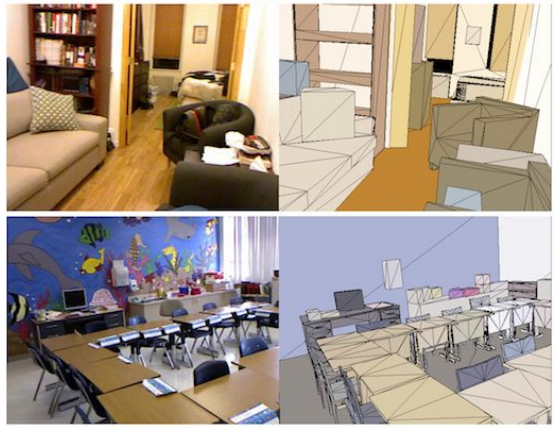
\includegraphics[width=1.0\columnwidth]{guo.png}% 
%     \figcaption{Representation of objects in the NYU dataset, provided from \cite{guo-iccv-2013}.
%     Not a perfect representation but perhaps reasonable to some extents.}% 
%     \label{fig:guo_labels}% 
% \end{figure}


\subsection{Database of CAD models}
Use the database from Fisher \ea \cite{fisher-siggraphasia-2012}.
1600 CAD models, each depth-rendered from 42 viewing angles using OpenGL.

\subsubsection{Potential test datasets}
\begin{itemize}
\item Create our own KinFu dataset
\item Kaparthy \ea --- would probably have to re-render their meshes.
Also don't have the TSDF etc. Lots of problems
\item NYU dataset --- classic dataset. Potential ground truth labels from \cite{guo-iccv-2013} (figure \ref{fig:guo_labels}) or \cite{kim-iccv-2013}.
\item \cite{fisher-siggraphasia-2012}, use their synthetic scenes (great for a first pass!)
\end{itemize}

% \begin{figure}
%     \centering% 
%     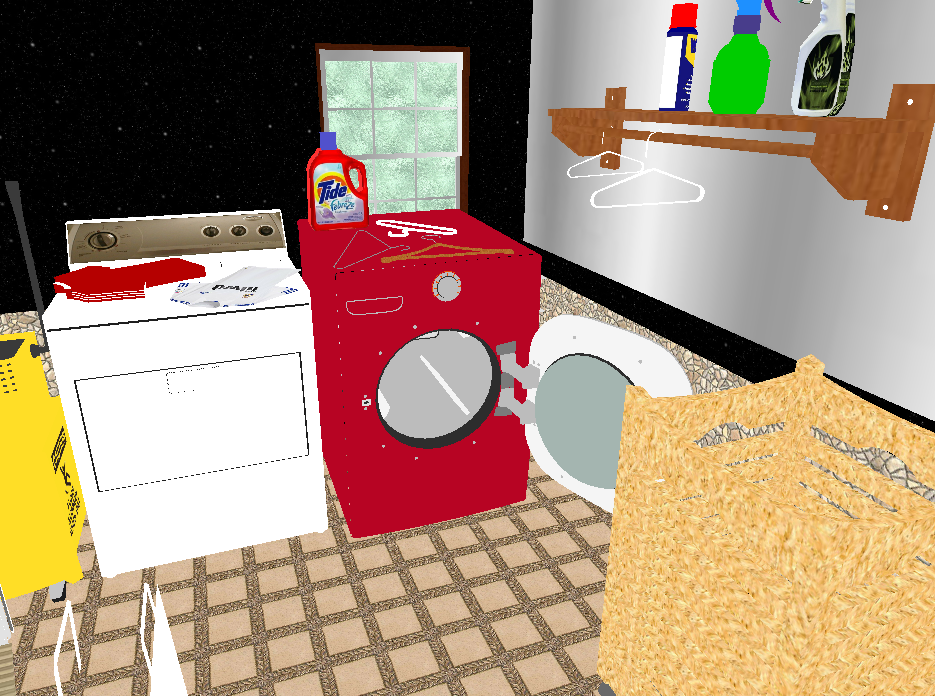
\includegraphics[width=1.0\columnwidth]{synth_scene.png}% 
%     \figcaption{One of the user-created synthetic scenes from \cite{fisher-siggraphasia-2012}.}% 
%     \label{fig:fisher_scene}% 
% \end{figure}

\section{Future work}

- Implicit voxel occupancy
- GPU
- 3D object models where they are known
- make splits in forest based on distance between cluster centers...  

\section{For supplementary material probably:}
But these could also come into the main paper:
\begin{itemize}
\item Reprojecting the depth image into the colour camera
\item Smoothing - both citations
\item Types of edges (depth, colour, occluding etc)
\item The method for finding depth edges
\end{itemize}

% \section{Acknowledgements}
% Peter Gehler
% Malcolm
% Neill
% Prism group
% Tom
% Peter
% Yotam


{\small
\bibliographystyle{ieee}
\bibliography{bibtex/strings.bib,bibtex/main.bib,bibtex/crossrefs.bib}
}

%\printbibliography


\end{document}